\chapter{The Tablet Method}
\label{chap:Tablet}

\textit{The work presented here has been presented previously as an oral presentation at AIC 2016 \citep[p. 125]{garside_estimating_2016}\footnote{Abstract available: \doi{10.6084/m9.figshare.4269680.v1}} and as a poster presentation at ECVP 2017 \citep[p. 93]{niko_busch_european_2017}\footnote{Poster available: \doi{10.6084/m9.figshare.5478493.v1}}}

\section{Summary}

The principal aim of this piece of work is to explore a novel method for colour constancy experiments, which allows for experiments to be performed in real and complex environments, in order to better understand colour constancy outside of a laboratory environment. The \gls{SAPS} method uses a tablet computer to present a spatial version of an achromatic point setting task. 

The key concerns are whether the proposed methodology can: a) present a stable stimulus across disparate environments, b) record differences in the state of chromatic adaptation, and c) be suitable for naive observers following minimal instruction. 

On each point, the method is shown to be moderately successful, with caveats, and suggestions are provided for improvements upon the current design. Such a methodology could be used to investigate the effect of multiple cues, conflicting cues and cues which cannot easily be reproduced in a laboratory environment.

Code and data are provided: \url{https://github.com/da5nsy/SAPS/}.

\newpage

\section{Introduction}

To further our understanding of colour constancy, investigators have traditionally designed well-controlled experiments where the number of variables is greatly reduced compared to a real-world environment. This allows investigators to carefully query the impact of any individual variable, or the interplay of a small number of variables. 

For example, a common stimulus-type used in such experiments are `Mondrian' patterns, arrangements of flat and unmoving overlapping coloured paper rectangles, see Figure \ref{fig:mondrian} \citep{hurlbert_colour_1999}. Consider also the experiments of \citet{kraft_mechanisms_1999} where objects representing potential colour constancy cues such as a tin-foil covered cone (specular highlights) were removed from a neutrally coloured box one-by-one in order to probe their relative usefulness as cues for colour constancy (see Figure \ref{fig:KraftBrainard}).

\begin{figure}[htbp]
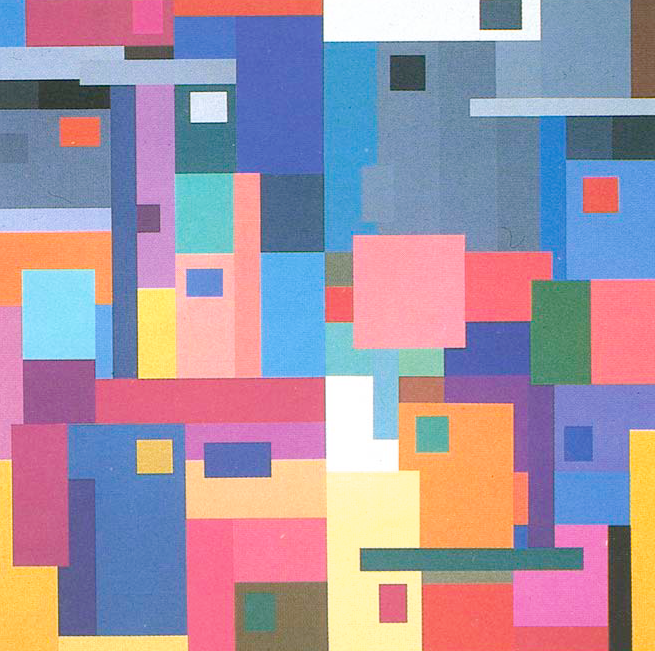
\includegraphics[max width=\textwidth]{figs/tablet/mondrian.png}
\caption{An example `Mondrian', reproduced from \citet{land_recent_1986}.}
\label{fig:mondrian}
\end{figure}

\begin{figure}[htbp]
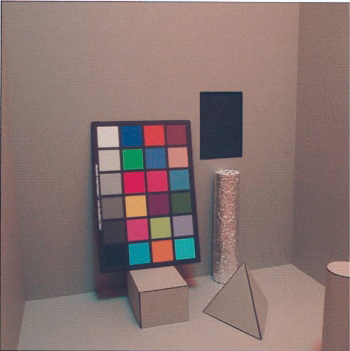
\includegraphics[max width=\textwidth]{figs/tablet/KraftBrainard.png}
\caption{A colour constancy experiment investigating the roles of different potential cues, reproduced from \citet{kraft_mechanisms_1999}. Objects within the scene were carefully selected such that the inclusion or removal or specific objects would allow or exclude the possibility of using a specific mechanism (local adaptation, spatial mean of the image, adaptation to the most intense region) to perform colour constancy.}
\label{fig:KraftBrainard}
\end{figure}

It is clear that these set-ups are much reduced in their complexity compared to a natural scene. Simple experimental stimuli allow for clear questions to be asked, and for those questions to be answered with statistical strength. Such research is valuable, but the results cannot always be extrapolated to other types of stimuli and different environments. The use of simplified stimuli risks overlooking unknown scene attributes, and the human behaviours which may be reliant on them. %LM: Ref Beau Lotto book
Experiments often find that colour constancy in lab environments is never `complete' \citep{murray_almost_2006,foster_color_2011}; is this representative of real world behaviour or could this result be due a lab environment failing to deliver all the cues available to an observer in a natural environment? Recent technological advances have enabled experimenters to reproduce natural scenes with increasingly accuracy and comprehensiveness \citep{heasly_rendertoolbox3_2014}, but the number of variables in real scenes is practically infinite, and whilst our ability to reproduce a scene increases over time as technology develops, we only reproduce what we deem important at the time. Using a real-world environment would allow for processes to occur as they do naturally, in the environment for which these processes are presumably optimised (See \citet{kelly_chips_2018} and \citet{shepard_perceptual_1992}). The ability to move away from the lab environment also allows us to run experiments in specific locations of interest, such as museum spaces.

There are at least two clear challenges to the use of natural environments for scientific study; the inability to control target variables, and the influence of uncontrollable or uncontrolled non-target variables. The first challenge may be surmountable; depending on the variable in question it might either be controlled by force, or over time natural variability may provide the required experimental range. The second may be insurmountable but, depending on the specific situation, it may be permissible to consider uncontrolled variations simply as sources of experimental noise. Further challenges arise where connections exist between target and non-target variables, or where the influence of the non-target variables dwarf the effect of the target variable.

One further challenge: it is rare for an experiment in a real-world environment to not intrude onto that real-world scene and change it in some way. The only true solution to this problem would be to consider unannounced observation of a natural behaviour as the only acceptable scientific method, which would be incredibly restrictive and impractical. A pragmatic compromise is to design an experiment such that it modifies the environment of the observer minimally, and to consider carefully the impact that the experimental set-up may have upon observers. This is the approach which shall be taken here.

The method presented here is a variant of the `achromatic setting' method.\footnote{For overviews see %section X, or 
the section on `achromatic adjustment' in \citet{foster_color_2011} and `Matching to an internal standard' or `achromatic setting' in \citet{smithson_sensory_2005}.} The achromatic setting method requires an observer, under specific conditions, to adjust the chromaticity of an item in their visual field such that this item appears achromatic. Changes in selected achromatic point (in colour space) are thought to represent general adaptive shifts. For example, an observer in an environment lit by a chromatic illuminant would be expected to pick an achromatic point which is shifted towards the chromaticity of the illuminant, compared to the achromatic point which they might select in a more neutral environment. This is often practically achieved by having the `object' be an area of a computer screen, and have it controllable in two or more chromatic dimensions (such as relative amounts of unique red/green and blue/yellow). 
%LM: refernces

In the \gls{SAPS} method, as presented here, a tablet computer is given to an observer to hold as is comfortable to them, and upon this computer an isoluminant slice through a nominally perceptually uniform colour space is presented, from which they are requested to select (by touching upon the screen with a finger) the point which they deem to be most achromatic (the specific phrase `grey-est or least colourful' is employed in order to make the task suitable for non-colour-scientist observers). The term `spatial' is used since the user provides information by making a spatial selection which directly corresponds to a colour choice, where in other methods abstract sliders or knobs may be used to alter the chromaticity of a static object.

To minimise the effect of the presentation of chromatic scenes upon the viewer, which may influence an observer's state of chromatic adaptation, this process is repeated a number of times with the area of colour space which is presented varying, through random rotation about the luminance axis, and random offsetting through both dimensions of the chromatic plane.

The rest of this chapter shall describe the method in more detail, and some experiments performed to explore the potential abilities and limitations of this method.

\section{Research Questions and Hypotheses} \label{sec:qandhyp}

\subsection*{Hypothesis 1: The \gls{SAPS} method is suitable for colour constancy experiments}

To be fit for performing colour constancy experiments, this method needs to:

\begin{enumerate}[label=\Alph*.]
    \item \label{list:hyp1a} \emph{Provide a relatively environment-agnostic stimulus.} 
    This experimental method relies on the assumption that the tablet display delivers a stimulus with identical physical properties to the observer independent of environment, with no effect of ambient illumination. In practical terms, this means that the tablet must not be affected by reflection, either at the glossy surface of the tablet display, or at reflection at any other level of the display architecture, to the extent that this has a non-negligible impact upon recorded data. If it is found that this is not the case, the tablet would need to be characterised separately for each environment.
    \item \label{list:hyp1b} \emph{Collect meaningful data.} 
    One would expect this to be indicated by small intra-observer variability (not recording a change where there is presumably none), and reasonable inter-environment change (recording a change where there is presumably a change). It would be expected that these changes would be in line with previously published results. An implicit assumption is that an observer's achromatic point will align with the chromaticity of the ambient illuminant.
    \item \label{list:hyp1c} \emph{Additional aim - Be suitable for naive\footnote{In this instance by `naive' I mean non-colour-scientist (a large number of colour vision experiments have been run only with colour scientists as observers and it is possible that this has biased results) and untrained (it is relatively common for this type of experiment to require extensive training upon a colour naming system such as The Munsell System of colour, by which participants are asked to report the appearance of a test object.)} observers.}
    This would reduce the amount of time and effort required to run experiments, and allow for the collection of data from participants less likely to be biased through task expectation. It also means that the demographic group of observers is less likely to be 
    WEIRD (`Western, Educated, Industrialized, Rich, and Democratic', \citep{henrich_weirdest_2010,brookshire_social_2013,justsaysinweird_just_2019}), white, and undergraduate.
\end{enumerate}

\subsection*{Hypothesis 2: \gls{ipRGC} activation affects perceptual white point.}
Primarily as a proof of concept for this methodology, but also to assist in answering other research questions posed within this thesis, an experiment was performed whereby observers made achromatic selections under a selection of colorimetrically metameric illuminants where there was a melanopic contrast between illuminants.
If \glspl{ipRGC} play a role in colour constancy we would expect to see a distinction between the responses recorded under the different illuminants. 

\section{Experimental set-up and methodology}

Three separate experiments were performed. These are described in Section \ref{sec:SAPS_exp}.

\subsection{Participants}

\subsubsection{Selection of participants}

The participants for Experiment 1 (Section \ref{sec:SAPS_exp1}) were the author, one of the author's academic supervisors (KC) and a technician at the laboratory (TS).

For Experiment 2 (Section \ref{sec:SAPS_exp2}), 58 observers were selected randomly from museum visitors. A visitor would be approached by the experimenter (the author) and asked whether `they would be interested in taking part in a colour vision experiment'. Those who replied positively were verbally informed of the ethics details for the study, the principal parts of which were: that no identifying information would be recorded, that the experiment carried no risks greater than those associated with normal use of a tablet computer, that observers were not paid or otherwise incentivised to take part, and that the task would take roughly ten minutes. A verbal description of the ethics details for this experiment was provided rather than the more traditional paper version to avoid providing the observer with a white reference immediately prior to the experiment. This study was approved by the \gls{UCL} Ethics committee (Project ID Number: 9357/001), application attached as Appendix \ref{app:ethics1}. In accordance with the ethics approval granted for this project, people under the age of 18 were only invited to participate under the supervision of a parent/carer.
% number, age and sex here? !!!!!!!!!

For Experiment 3 (Section \ref{sec:SAPS_exp3}), nine participants (5 female, 4 male, ages not recorded) were recruited from the author's friends and family (including one academic supervisor, LM), with the hope that this would assure attendance and motivation and to take advantage of short-notice availability of the experimental space. Participants were informed of the ethics details for the study in advance of attending. Ethics approval was provided following the amendment of the aforementioned ethics application (9357/001), attached as Appendix \ref{app:ethics2}.
% number, age and sex here? !!!!!!!!!

\subsubsection{Instructions to the participants}

The observer was instructed to hold the tablet such as was comfortable for them to do so, upon which the first trial of the experiment was already visible. They were instructed to `touch the grey-est, or least colourful, point on the screen'. Upon touching the screen, the stimulus would be replaced with a new stimulus. This new stimulus was a new subsection of the full stimulus image (See Figure \ref{fig:Stimulus}) which had been randomly rotated and offset (further information provided in Section \ref{sec:stimuli}).

\begin{figure}[hbtp]
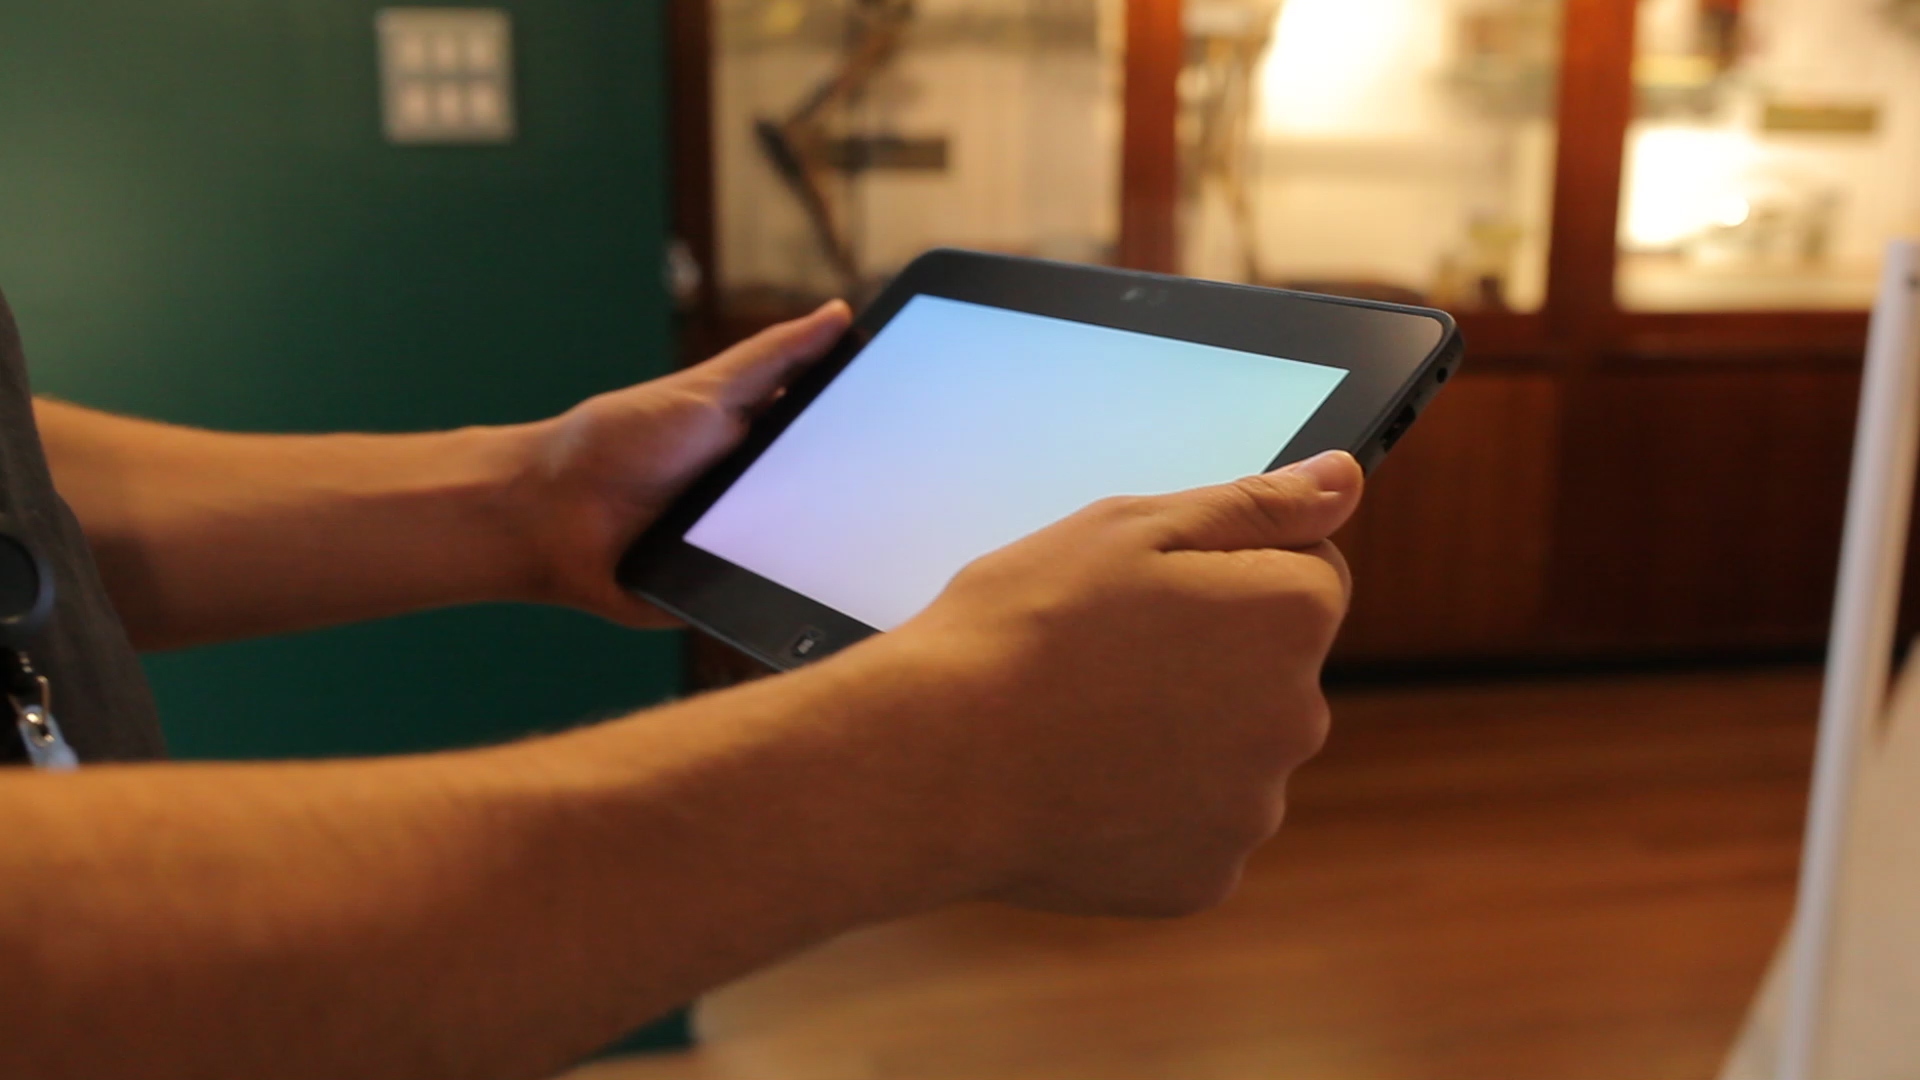
\includegraphics[max width=\textwidth]{figs/tablet/MVI_3213-1.jpg} % E:\Pictures\2016\2016-10-14
\caption{A participant (the author) holding the tablet with a stimulus on screen.}
\label{fig:grant_demo}
\end{figure}

Most observers seemed to find this task difficult for the first stimulus (appearing confused and often verbally expressing difficulty), but within the first few stimuli seemed to develop an increased comfort and ease with the task, resulting in a decreased response time (Figure \ref{fig:mediantime}). At this point the observer was told that there would be thirty trials. No training was provided, and no runs were excluded as training runs. One stimulus was forced to have identical rotation and offset to an earlier stimulus, in order to assess intra-observer variation (see Section \ref{sec:exclusion}).

\begin{figure}[hbtp]
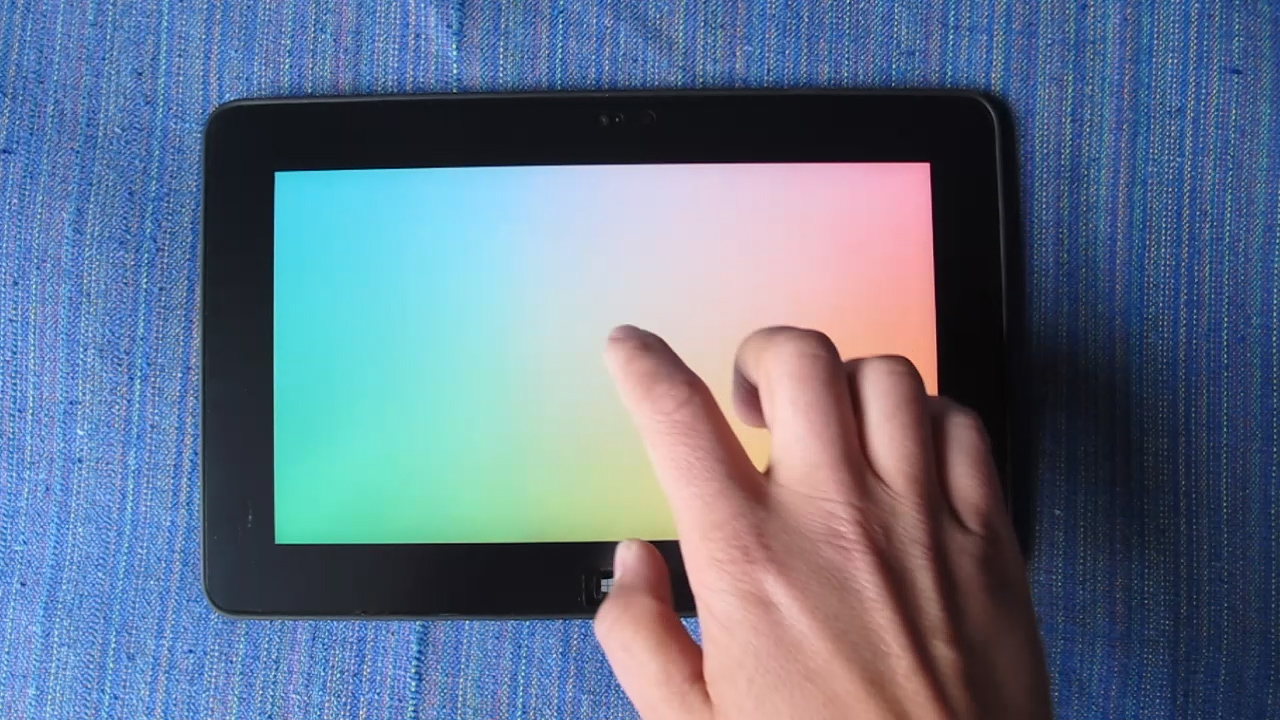
\includegraphics[max width=\textwidth]{figs/tablet/MVI_3889-4.jpg} % E:\Pictures\2016\2016-10-18
\caption{A stimulus displayed upon tablet and finger in motion towards subjective point of achromacy.}
\label{fig:finger}
\end{figure}

Following the thirty trials, a secondary task was presented to observers, designed to characterise their touch input. This task features a 2x2 checker board pattern upon a black background (See Figure \ref{fig:checker-board}). Observers were instructed to touch the centre of this checker board. Upon registering a touch, a new checker-board would be presented, of the same attributes but modulated in position in the same way as the main stimulus. This stimulus is presented 10 times. This data was later used to calibrate touch input, and to ascertain the amount of measurement uncertainty derived from touch input. %!!!!!! This is doing weird formatting, check before submission

\begin{figure}[hbtp]
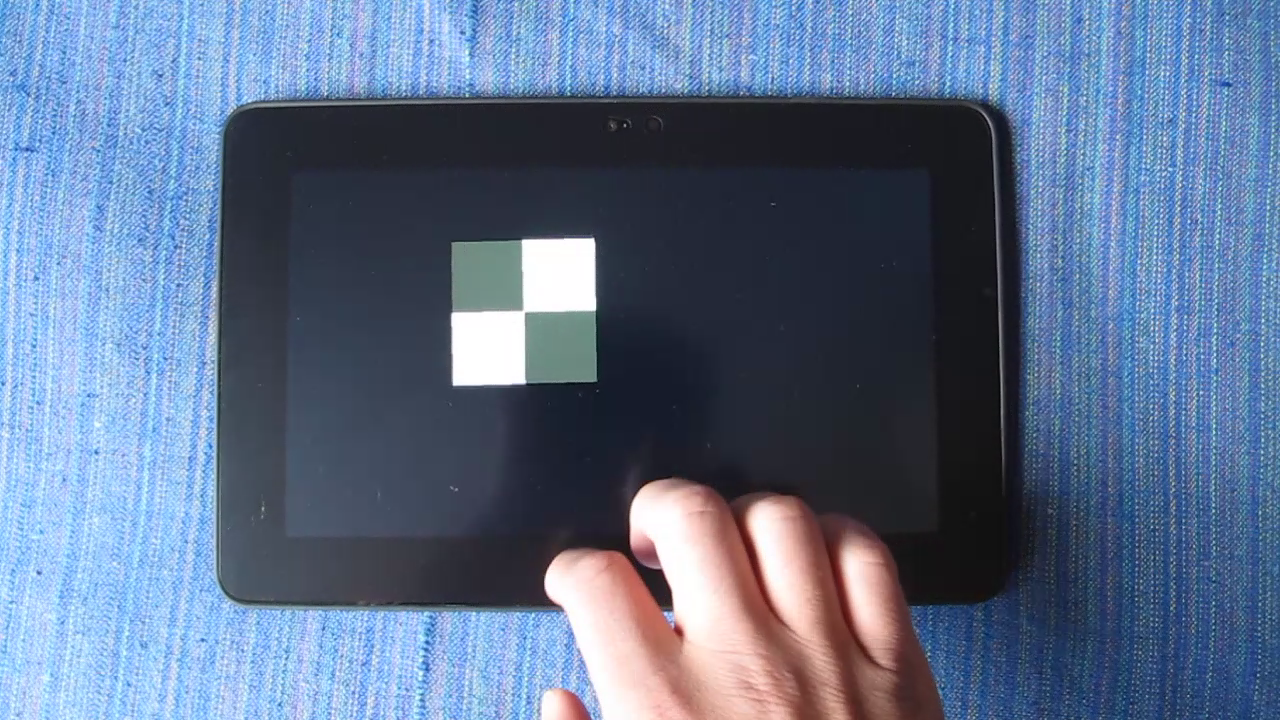
\includegraphics[max width=\textwidth]{figs/tablet/checker_board.png} % E:\Pictures\2016\2016-10-18
\caption{Photo of checker-board task. Participant is requested to touch centre of the checker-board pattern.}
\label{fig:checker-board}
\end{figure}

% \clearpage %currently ending up with a single line which looks dodgy, check later %!!!!!!!!!!!!!

%Doing this without incentive for participants meant that it was rushed (?)

\subsection{Stimuli} \label{sec:stimuli}

\subsubsection{Selection of stimuli colour space}

The stimulus presented to observers was an isoluminant plane (in CIE L*) through CIELUV colour space. CIELUV was chosen, over CIELAB or CIECAM02 for example, since it has an associated object colour space, which allows for comparisons between the chromaticity of light sources and the chromaticity of selections to be made\footnote{Some preliminary runs of the experiment, performed at The UCL Grant Museum, used a stimulus defined in CIELAB colour-space instead, before later changing to CIELUV for the reason above.}. 

\subsubsection{Generating the stimuli}

The stimulus was specified as: L*: 60 uniformly across field, u*: ranging linearly from -50 to 50 from one side of the field to the other, and v*: as for u*, but along the orthogonal axis, so that the stimulus was of uniform lightness and smoothly changing hue and chroma. The full stimulus image (Figure \ref{fig:Stimulus}) was 2188 x 2188 pixels; this is larger than the pixel dimensions of the chosen screen (1366 x 768, Section \ref{sec:spec}) to allow for the stimulus to be rotated freely and offset by up to a third of the image in any direction before the edge of the image is encountered. 

The stimulus was specified with the above attributes in a matrix within \gls{MATLAB}\footnote{Code: \url{https://github.com/da5nsy/SAPS/blob/21940bb6ed9d0e37d88e1b655f4919d73431743a/experiment/stimulusGenerator002.m}}. CIELUV values were converted to XYZ tristimulus values, with reference white set as the XYZ tristimulus values of the display at maximum white (with screen protector), as measured with an Xrite i1 device (shown in Figure \ref{fig:gamut}). Linearisation was achieved through the use of a look-up table, computed by spline interpolation of the measured outputs at 15 pixel %(KT: pixel drive value?)
value increments from 0 to 255 for each channel. The stimulus was then output as an 24-bit RGB tiff, which could be easily loaded and manipulated by the psychophysical stimulus presentation software PsychoPy \citep{peirce_psychopypsychophysics_2007}. %(Illustrate with flow diagram?)

\begin{figure}[hbtp]

\includegraphics[max width=\textwidth]{figs/tablet/stimulus.png}
\caption{Full stimulus image, from which subsections were selected and presented as stimuli. Note that no effort has been made to correct this image for printing, and so it is best considered as only a rough approximation. It may be possible to see the vertical line on the left where the sRGB gamut boundary is reached; this is further described in Figure \ref{fig:stimchan}.}
\label{fig:Stimulus}
\end{figure}
% Copied and pasted from original psychopy folder. Could regenerate using stimulusGenerator002.m

\subsubsection{Presenting the stimuli} \label{sec:presenting_the_stimuli}
A program was written in PsychoPy\footnote{\url{Code:  https://github.com/da5nsy/SAPS/blob/21940bb6ed9d0e37d88e1b655f4919d73431743a/experiment/SpatialAchromaticPointSetting_0940_Grant.py}} that presents the stimulus 30 times%LM: need discussion of why 30 times
, with random rotation and random offset in the horizontal and vertical dimensions of between -1/6 and +1/6 of the respective dimension. Thus `objective grey', where [u*,v*] = (0,0), was always within the central third (in each dimension) of the screen. This program saved details of the stimulus offset and rotation (`dpX', `dpY' and `ori'), co-ordinates of observer selected point (`x-co\_raw', `y-co\_raw', and also `direction\_raw', `magnitude\_raw'), and time taken to make selection, measured since last selection (`toc\_raw').

The effect of rotation and offset was such that on each stimulus presentation the observer saw a stimulus that appeared somewhat different to the previous stimulus, but still hopefully included their perceptual achromatic point. %The rotation and offset can be illustrated by plotting the chromaticities present in any one stimulus presentation, as in figure X. %!!!!!!!!!!!!!!!!!!!
Plotting the chromaticities present across a full run of 30 trials yields Figure \ref{fig:practical}, where it can be seen that the rotation results in a roughly circular spread of chromaticities, and the rotation and the offsetting together result in a gradient of likelihood of presentation which is high at the centre of the full stimulus and lowest at the edges of the full stimulus. This gamut distribution is referred to further in the text as the `practical gamut'.

% Single shot figure needed

% \begin{figure}[hbtp]
% \includegraphics[max width=\textwidth]{figs/tablet/????}
% \caption{A representation of the chromaticities present in a single stimulus. Note that the gamut is not rectangular for 2 reasons: firstly, because CIELUV is not a linear transformation of CIE u'v' , and secondly because for this particular stimulus, the bottom left corner (as presented above) intersects with the display gamut boundary, resulting in a gamut compression to that corner.}
% \label{fig:?????}
% \end{figure}


\begin{figure}[hbtp]
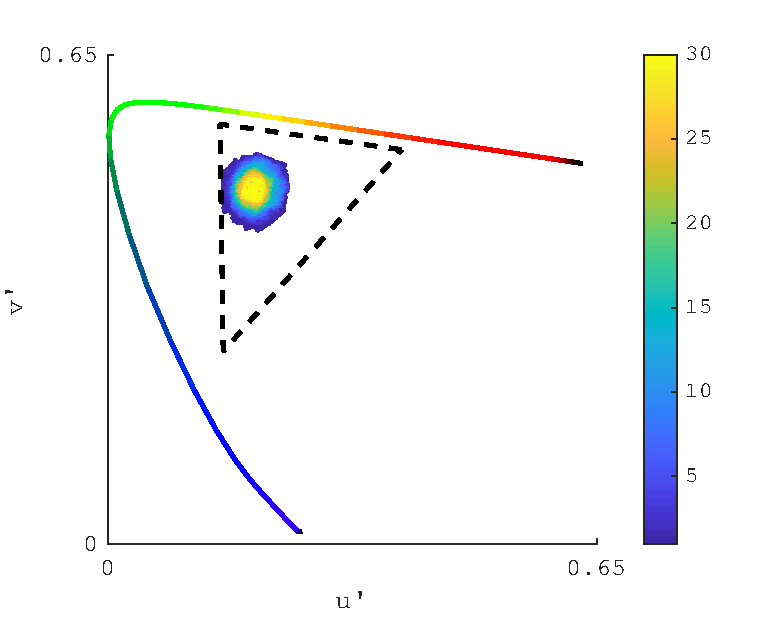
\includegraphics[max width=\textwidth]{figs/tablet/practical_gamut.pdf}
\caption{The `practical gamut'. This plot shows the relative frequency that chromaticities are actually presented, within the device gamut (more fully described in Figure \ref{fig:gamut}). The highest number of times a particular chromaticity can be presented is 30, since there are 30 trials in a typical run. Chromaticities falling towards the objective white point of the stimulus are presented every stimulus, whereas those further away from the centre of the stimulus are presented less frequently. On the left-hand side of the cluster it can be seen that the gamut boundary is reached.}
\label{fig:practical}
\end{figure}

\subsubsection{Limitations of the stimuli} \label{sec:limitations}
Under the current set-up the stimulus is to some extent fixed; each stimulus is a subsection of a single complete stimulus image (Figure \ref{fig:Stimulus}). This means that an observer can at no point select a chromaticity that is not present in the full stimulus, and they will less often have the option to select a chromaticity which falls towards the boundary of this stimulus space than they would be able to select one at the centre of this space, due to the nature of the rotation and offset described in Section \ref{sec:presenting_the_stimuli} (See Figure \ref{fig:practical}). 

When designing the stimulus it was assumed that the stimulus would cover a large enough area of colour-space to allow for any selection that an observer would reasonably care to make (the stimulus would include an achromatic area surrounded by areas which under no situation would be deemed achromatic). Later analysis (for example, see Figure \ref{fig:PAMELA_DG_results} where an illuminant falls far outside the practical gamut) showed that this was not the case, and that it was not unusual for an illuminant that appeared entirely neutral to fall outside of the response-space. I had underestimated the power colour constancy!

This limitation leads to a pattern in the data which I shall refer to as `smearing', so called because when the desired selection point is outside of the practical gamut, or even close to the edge of the gamut, the closest possible points which are available for an observer to select will fall upon a line between the objective white point (the white point of the display) and the true desired selection point, thus the data is smeared between the point which an observer actually wants to select, and the objective white point. This is discussed further is Section \ref{sec:bounding}, where amendments to this experimental method are proposed which might limit or remove this effect.

A visual example of this can be given by considering the results of an amended experiment where the same stimulus was presented but the question changed to `touch the X-est point on the screen' where X was red, green, blue or yellow. See figure \ref{fig:basement_rgby_test}. This is a more extreme case than a white-appearing light source outside of the practical gamut but it is thought that the effect upon the data would be similar.

\begin{figure}[hbtp]
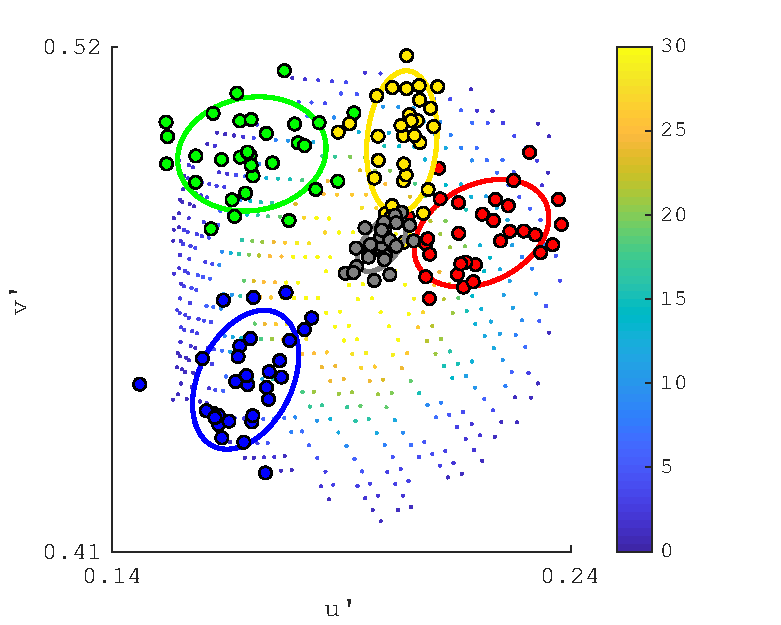
\includegraphics[max width=\textwidth]{figs/tablet/basement_rgby_test.pdf}
\caption{Results from an amended experimental paradigm to demonstrate `smearing'. The observer was asked to `touch the X-est point on the screen' where X was red, green, blue or yellow. A normal run of the experiment was conducted under the same conditions at the same time to provide a baseline condition.\\ 
The experiment was performed in the basement of the Chadwick Building (Section \ref{sec:Chadwick}) with the author as observer.}
\label{fig:basement_rgby_test}
\end{figure}

A broader limitation, which applies to all screen-based experiments, is that regardless of the gamut of the stimulus used (here `practical gamut') we are operating within a larger fixed gamut, shown within Figures \ref{fig:practical} an \ref{fig:gamut}. It can be seen in Figure \ref{fig:practical} that our chosen stimulus gently nudges the left-hand gamut boundary of the screen. This can be thought of as a request for colours which are less red than is possible using this specific display.

The effect of this could be reduced by choosing a screen with a particularly large gamut. A drastic alternative might be to consider a reflective screen device (such as a Kindle or other e-reader/e-ink device) but this would immediately fail Hypothesis 1A (\emph{`Provide a relatively environment-agnostic stimulus'}) and so the device would need to be characterised within each new environment, which reduces the appeal of this method considerably.

\subsubsection{Touch input characterisation} \label{sec:touch}
The checker-board stimuli (Figure \ref{fig:checker-board}), included to allow for fine spatial calibration for individual observers' touch input, was generated by running the main experimental script again but with the stimulus file path replaced with a simple pattern generated within PsychoPy.

I hypothesise that any shifts in touch input would be the result of one or both of two potential influences: personal finger offset and general hardware calibration. By the former I refer to the fact that whilst a finger is considered to be a relatively discrete unit, controlled with presumed dexterity and accuracy, the specific part of the finger which touches the screen will vary from person to person, with each person exhibiting a reliable bias. By the latter I refer to the fact that it is highly possible for there to be a `fairground gun effect', whereby the hardware introduces a reliable bias due to calibration misalignment, which affects every observer equally.

Performing a calibration of each observer's data based on this individual characterisation allows for offsetting of both of these types of variation. 

\subsection{Specification of Tablet PC} \label{sec:spec}

Participants undertook the experiment upon a Dell Latitude 10 ST2 tablet computer (223x126mm active screen area, 1366x768 pixels) with `BROTECT' Matte Screen Protector (a thin adhesive, translucent, and matte screen protector). This tablet was chosen for its ability to run a Windows environment, and the screen protector was added to reduce the severity of specular reflections. The measured gamut of this device is shown in Figure \ref{fig:gamut}, with the gamut of sRGB for comparison.

\begin{figure}[hbtp]
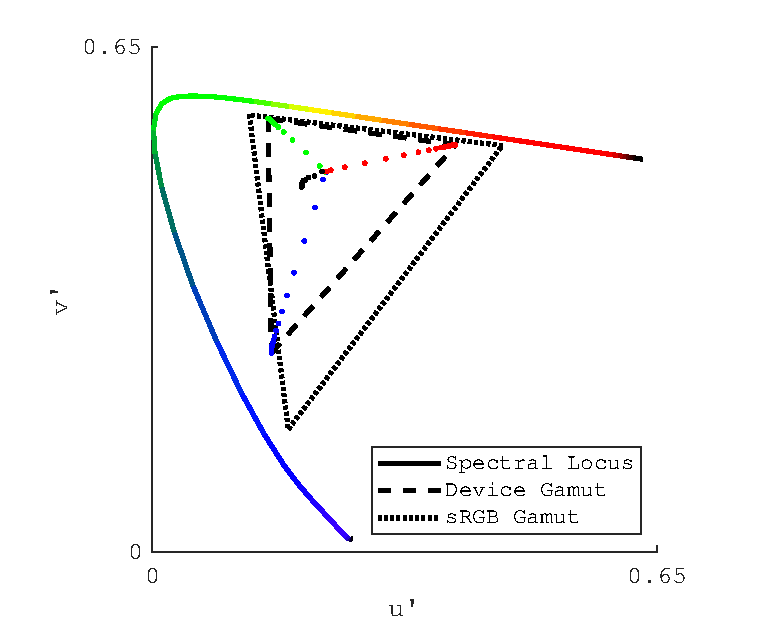
\includegraphics[max width=\textwidth]{figs/tablet/gamut.pdf}
\caption{The display gamut, plotted in CIE u'v' space. Red, green and blue dots indicate chromaticities of single channels at pixel values from 0 (central values) to 255 for each respective channel. The black dots are the chromaticities achieved when the pixel values are kept in line for each channel. This can be described as the native white point of the display, and can be seen to drift leftwards and then downwards as pixel values increase.}
\label{fig:gamut}
\end{figure}
% Generated using the 'Plot gamut' section of SAPS_TabletCharacterisation.m

\subsubsection{Impact of ambient illumination} \label{sec:ambient}

A key requirement in this methodology is that the display device remains roughly colorimetrically stable across a range of lighting environments (see \hyperref[list:hyp1a]{Hypothesis 1A}). This would only be true if the device produced the entirety of the light emanating from it in normal use. In reality, a small amount of light will be reflected from the surrounding environment. This may be reflected either at the surface layer of the screen (specular reflections) or at a lower level of the screen architecture. Here we aim to quantify the amount of light reflected in this way, understand the impact that this has on this method, and seek to minimise this impact if possible.

It is assumed that specular reflections are clearly distinguishable to most users, and that users will automatically hold the device in such a way as to minimise their interference with the task. It is also assumed that the spatial nature of such reflections and the fact that they are not locked to the geometry of the screen (but rather move as the screen or observer moves) would further allow an observer to visually discount them and not confuse them for an output of the screen.

The key concern then is reflection at other levels of the screen architecture. Using the screen calibration framework \cite{berns_crt_1993}, this may be considered as an environment-dependent `offset', that is, a figure which is added to the output of the screen at all levels. It is assumed that this level is constant in an unchanging environment, and independent of the output of the screen. It therefore follows that this will have greatest impact on the chromaticity of the display at low luminances, where the amount of reflected light is high relative to the output of the display.

To consider whether such reflections exist for our specific set-up, telespectroradiometric measurements were taken of screen at varying pixel value levels (0 to 255, intervals of 15)\footnote{Code: \url{https://github.com/da5nsy/SAPS/blob/master/auxiliary_functions/tablet\%20characterization/calibration.py}} under 3 different lighting conditions, as described in Section \ref{sec:PAMELA}. One condition was repeated to assess measurement uncertainty. The measurement device used was a \gls{PR650}. 

Broadly speaking, at a pixel value of 0 one would expect that the illumination reaching the position of the observer depends almost entirely upon the illumination (entirely, if we assume that the black of the screen is uniformly spectrally reflective), whereas at maximum output (pixel values of 255 in all channels) the illumination reaching the position of the observer would be greatly more dependent upon the output of the device, hopefully with negligible influence of the illumination (so long as the illumination was below a certain threshold). The point of interest is therefore assumed to be the pixel value where the shift resulting from differing illuminants jumps from being non-negligible to negligible for our purposes.

\begin{figure}[hbtp]
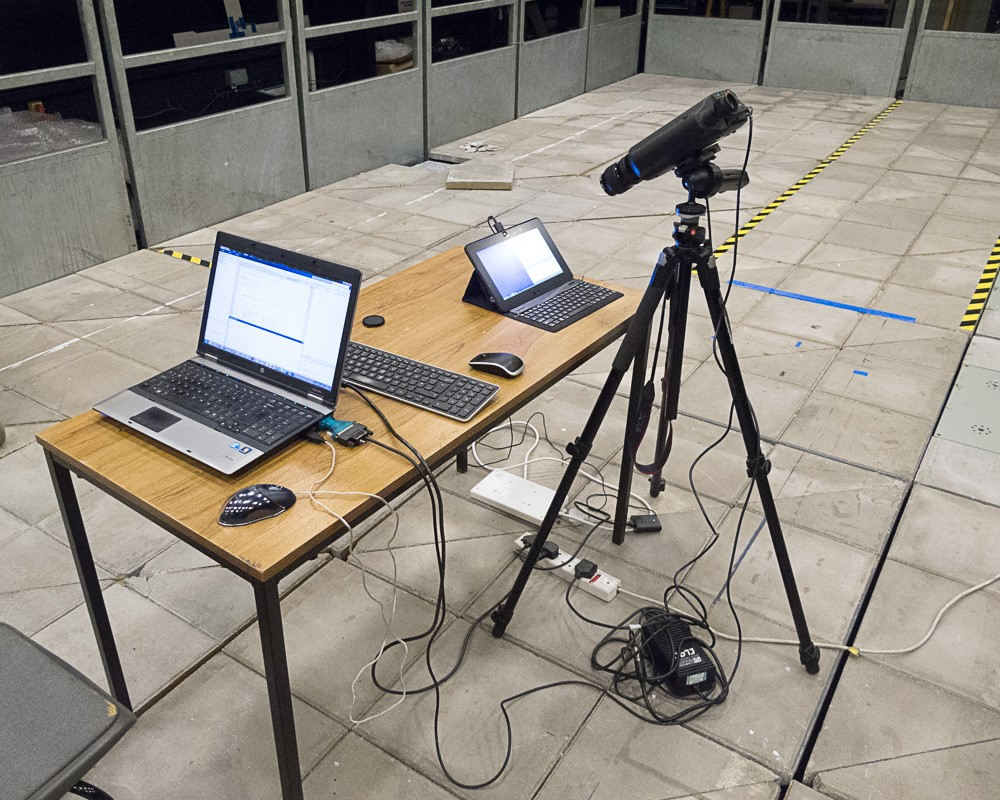
\includegraphics[max width=\textwidth]{figs/tablet/pamela_pr6501.jpg}
\caption{The measurement set-up at \gls{PAMELA}. PR 650 on right, with control PC on left, and tablet in the centre.}
\label{fig:pr6501}
\end{figure}

\begin{figure}[hbtp]
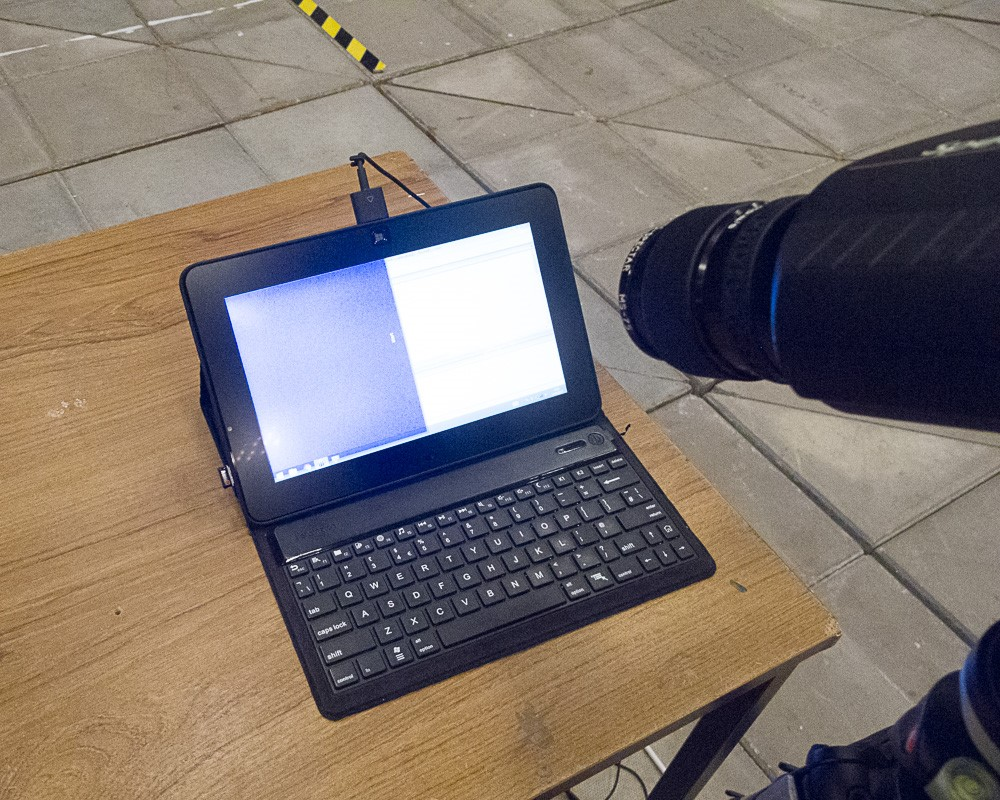
\includegraphics[max width=\textwidth]{figs/tablet/pamela_pr6502.jpg}
\caption{The measurement set-up at \gls{PAMELA}. The tablet computer, showing the characterisation routine (on the left of the screen). Note the specular highlight on the left of the tablet frame, reflecting the detail of one of the many \gls{LED} arrays overhead.}
\label{fig:pr6502}
\end{figure}

As shown in Figure \ref{fig:pr6503} it was found that for pixel values of 60 and below there was a considerable chromaticity variation between data from each lighting condition. This aligns with our expectation that the greatest effect would be seen at lower screen output levels.

\begin{figure}[hbtp]
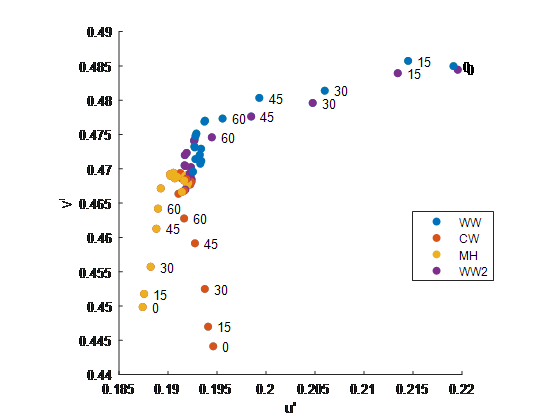
\includegraphics[max width=\textwidth]{figs/tablet/pamela_pr6503.png}
\caption{Chromaticity co-ordinates of measurements at different pixel values. It can be seen that the 0 values diverge greatly. They do not diverge in exactly the directions of the chromaticities of the light sources, which could either be due to measurement inaccuracy, or the base colour of the tablet may not be perfectly neutral. At higher pixel values the chromaticities start to converge at around [u',v'] = [0.193,0.47].} %would be nice to reproduce !!!!!!!!!!
\label{fig:pr6503}
\end{figure}

%LM: plot measured luminance vs pixel value

For values above 75 (inclusive), a conservative estimate for the maximum shifts in chromaticity due to variation between light sources (considering only those sources tested) would be roughly 0.004 in the u' axis, and 0.009 in the v' axis. These values are derived from visual inspection of the variation in values of chromaticity for readings taken of pixel values above 75. These figures could be considered baseline figures for classifying observed differences as likely to originate from genuine changes in observer state rather than lighting/stimulus artefacts.

It is noted that the variation between the repeated measurements, denoted `WW' and `WW2', is larger than might be expected; at high pixel values the chromaticities recorded under `CW', `MH' and `WW2' converge very well, but `WW' seems offset by roughly 0.005 units in a roughly north-east direction% KC wasn't keen on this, see what others say
in colour space. The cause of this is unclear. The cause could be the result of `warm up' (either in terms of an actual temperature dependency, or in terms of a device taking time to settle into a default operating mode after turn on) of either the screen or the spectroradiometer. It could also be the case that between measurements the angle of the screen relative to the spectroradiometer and that this was the cause of the distinction.

% ----------% This is all well and good but not required. 
% Consulting the spectral data for `WW' and `WW2' (Figure X%!!!!!!!!!!!
% ) we can see a systematic variation whereby for the initial `WW' run the recorded values for lower wavelengths are slightly lower, and the higher wavelengths record slightly higher values, when compared to the `WW2' data.

% % figure

% Another way of representing the above is to consider the effect that changing lighting has on the recorded spectral power distribution of light entering an aperture at the rough location of an observer's eye.

% % figure
% % [Caption: The recorded spectral power distributions, for each measured level of pixel value, under each of the 4 illuminations. Plots are limited to lower pixel values for attention.] Need to find a better way to present this

% Above, it can be seen that at lower levels of pixel value, the spectral power distributions are notably different between lighting conditions. Under `MH', for example, there is a noticeable difference in \gls{SPD} shape whereby at the lowest pixel values there is a peak around 470nm, which quickly fades from notice as pixel values increase. For `CW' in comparison, we can see that the 450nm peak is substantially higher at low pixel values than at either of the `WW' measurements, suggesting that this light source provides additional power at these wavelengths.

% In all the cases above, the impact of such perturbations can be seen to fade rapidly with increasing pixel value.

% Now that we have considered the effect of lighting upon the tablet in a general sense, we must consider what effect would be had upon the rendering of our specific stimulus.

% %figure

Now I shall consider the impact of the above finding upon our specific stimulus. Figure \ref{fig:stimhist} shows the histogram of each channel within the full stimulus. Note that only the red channel has a significant number of pixels with values below 75 (with the blue channel having some values which come close), and so following from our observation that chromaticity was most perturbed by variations in lighting where the pixel value was below 75, this is the channel most likely to be influenced by the ambient illumination (though only in specific spatial sections of the stimulus image).

\begin{figure}[hbtp]
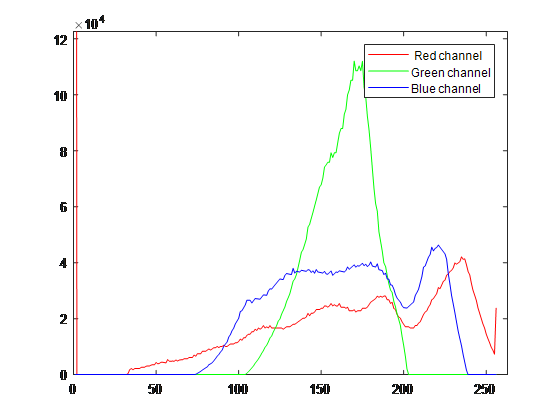
\includegraphics[max width=\textwidth]{figs/tablet/stimhist.png}
\caption{Histogram for the different channels in the full stimulus image.} %would be nice to reproduce !!!!!!!!!!
\label{fig:stimhist}
\end{figure}

Note also that whilst the blue and green channels possess no pixels at either end of the pixel value range (0/255), the red channel possesses both, suggesting that a gamut boundary is reached at both extremes for the red channel. A large number of pixels in the red channel are at 0, with a small number at 255, representing points at which the sRGB gamut is reached. From \ref{fig:stimchan} it can be seen the zero values are located on the far left of the stimulus, in the strongly blue/green area, and that the 255 values are located in the bottom right hand corner, in the strong red/pink area.

\begin{figure}[hbtp]
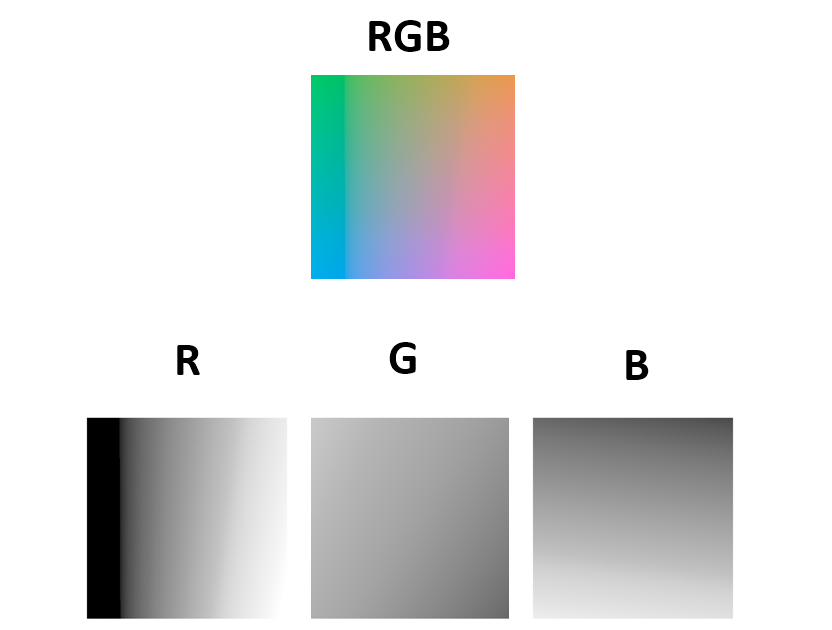
\includegraphics[max width=\textwidth]{figs/tablet/stimchan.png}
\caption{A breakdown of the stimulus image by channel. Here it can be seen that for the red channel, we reach the edge of the range, with a black bar being visible vertically on the left and a white corner (just about) visible in the bottom right. This translates, in the RGB image, to a bar on the left which appears to only vary in blue/green and an area in the bottom right which does not vary in red-ness. Note that the reproduction here is crude and only roughly estimates how the stimulus would appear during the experiment.}
\label{fig:stimchan}
\end{figure}

In summary, measurements taken lead us to conclude that influence of the ambient illumination, for the illuminations we have tested, has a minimal effect on the presentation of the stimulus as defined in this experiment (up to 0.004u' and 0.009v'). The greatest effect will likely be upon the sections of the stimulus where the pixel value falls below 75, as happens in specific areas of the red channel image. These chromaticities will not be often presented since they fall at the edge and corner of the full stimulus. %would be nice to add the full stimulus onto one of the gamut diagrams !!!!!!!!!

%It is likely that these areas of the stimulus are unlikely to be ambiguous in colour appearance to an observer, and so any slight difference between the chromaticity ideally presented, and the chromaticity actually presented, is likely to have only a minimal impact.
% They have variation in the other channels, just not red

It would be possible to create a stimulus which did not reach the gamut boundaries, and which does not include pixel values below a certain value for any channel. However, if using the same hardware, the trade-off would be that a smaller section of colour space would be presentable, and this would have two knock-on effects; the task would be harder (the stimulus would be less saturated), and the results would be more tightly bounded (the observer would not be able to select more chromatic points). For further discussion of `bounding' see section \ref{sec:limitations}.

The measurements taken here are limited in scope by the fact that the effect of ambient illumination is likely linked to the overall level of ambient illumination; it is likely that in much brighter conditions the illumination would have a greater effect on the chromaticity of the stimulus. This should be considered when assessing data collected in very bright conditions.

It also seems noteworthy to explicitly consider that we have assumed a linearity of sorts in asserting that there is likely to be a colorimetric effect where pixel values in any one channel drop below a threshold value. In reality, our tests show that chromaticity is affected when pixel values of all three channels drop below a threshold value, and it is a conservative assumption to assert that there is a risk when a single channel drops below this threshold value. It is quite possible, for example, that where values in the red channel drop below the threshold, if the surrounding blue and green pixels are being driven at high values, that bleed may limit the practical impact upon overall chromaticity.

% Is it additive?
% LM recommendation: Go back to basics: consider the ambient lighting, and the lighting produced by the emissive display, Compute, predict, compare. Plot gamuts

\subsection{Data Analysis}
\subsubsection{Processing Pipeline} \label{sec:processing}

The data was analysed in \gls{MATLAB} using the following pipeline:
\begin{enumerate}
\item Data loaded into \gls{MATLAB} from an excel file
\item Spatial touch points calibrated using touch characterisation data
\item Spatial data converted into chromaticity data
\item Data graded for performance and exclusions applied where appropriate (see Section \ref{sec:exclusion}) 
\item Data plotted either as:
\begin{enumerate}
\item Full dataset scatter
\item Standard deviation ellipse/line plotting\footnote{Based on code from: \url{https://stackoverflow.com/a/3419973}}.
\item Dataset mean plotting (where number of participants was large)
\end{enumerate}
\end{enumerate}

\subsubsection{Exclusion Criteria} \label{sec:exclusion}

In this task, a `good' performance is one where it seems an observer understood the given instructions well, and was able to act upon them. Such a performance should be indicated by data which suggests that an observer was able to repeatedly select their chosen chromaticity in spite of the spatial relocation of this chromaticity during the experiment. It is expected that observers will perform with differing levels of competence, due to a variety of reasons, e.g.: level of commitment/interest, visual/pointing ability, understanding of the task. It seems reasonable to exclude all data from any observer where some of that observer's data indicates that they have performed `less well' than a determined threshold.

A measure of performance could be computed by measuring variance in a dataset for each observer. In an ideal situation, an observer would select precisely the same chromaticity on each trial, and so the variation would be 0. More realistically, slight variance is expected, due to input imprecision, fuzzy boundaries of acceptability and `smearing' artefacts (see Section \ref{sec:limitations}).

Two simple methods for assessing this variability are readily available. The first involves calculating the standard deviation of data for each observer; either considering a single chromatic axis, both axes, an average of both axes, or considering a newly defined axis such as the axis of greatest or least variability. The second involves comparing data from unannounced repeat stimuli (within each observation run trials 3 and 8 were identical, and if an observer was performing the task effectively the difference in records for these two stimuli should be minimal). This second method shall be referred to as \acrfull{DBUR}.

The first method has the advantage that it considers the entirety of each dataset; whereas the second method requires that general assumptions about the entirety of an observer's data be made from only two data points. One disadvantage of the first method however, is that this measure would give a high value in the situation that there was a moderate or higher level of `smearing', since increased spread could result from a situation where an observer was very good at selecting their chosen chromaticity, but was unable to do so since that chromaticity was not always displayed. In contrast, the second method should be unaffected by this.

A further advantage of the first method is that a non-arbitrary threshold presents itself; that of the level of variability which would result from a run of the experiment where a hypothetical observer selected the exact same physical point on the screen for each stimulus. This would represent the best possible performance of an observer who was unable, or had no interest in, following a specific chromaticity, though of course it would not include any variability attributable to a touch input (though this could be artificially simulated). The second method presents no such intuitive definition for a threshold.

Both assume that an observer's state of chromatic adaptation remains stable across a run, which is not certain.

\begin{table}[hbtp]
\begin{tabular}{|p{0.5\textwidth}|p{0.5\textwidth}|}
\hline
\emph{Standard Deviation} & \emph{\acrshort{DBUR}} \\
\hline
Considers entire dataset & Requires generalisation from only two points per observer \\
\hline
Susceptible to `smearing' artefacts & Not affected by gamut boundary issues \\
\hline
Intuitive threshold: the SD of a `baseline' observer & No intuitive threshold \\
\hline
\end{tabular}
\caption{Comparison of exclusion criteria options.}
\label{tab:exclusion}
\end{table}

% I don't really do stats here...
% \subsubsection{Statistical Analysis}

% Data was considered in comparison to a baseline dataset, consisting of the results of a theoretical trial where an observer touched the spatial centre of the screen each time %(further details in section 5.1), 
% and a practical gamut which describes the frequency with which each chromaticity was presented to the observer. %!!!!!!!!!!! (See section 3.1 for further discussion of this).
% %Demo plots?

\subsection{Environments}

\subsubsection{UCL PAMELA} \label{sec:PAMELA}

\gls{UCL}'s \acrfull{PAMELA} (used for Experiments 1 and 3) consists of a large open space, enclosed within a light-proof warehouse, and is most often used for its customisable floor space, where small sections can be independently raised or lowered to recreate the spatial configurations of public spaces such as streets or railway platforms (see \citet{cheng_effect_2018} for example, and Figure \ref{fig:PAMELAobs1}). It is of interest to this project since it also has a customisable lighting rig comprising 44 addressable fixtures, each with 6 independent channels, which is controlled via a PC interface, and an additional high power white channel, which is on a separate control system. 

\begin{figure}[hbtp]
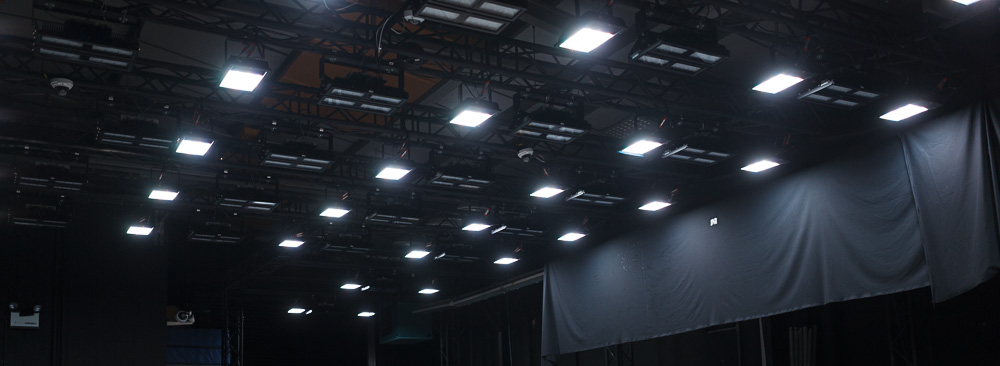
\includegraphics[max width=\textwidth]{figs/tablet/PAMELAlights1.jpg}
\caption{The fixtures mounted on the ceiling lighting rig at \acrshort{PAMELA}. Photo credit: Keats Webb.}
\label{fig:PAMELAlights1}
\end{figure}

\begin{figure}[hbtp]
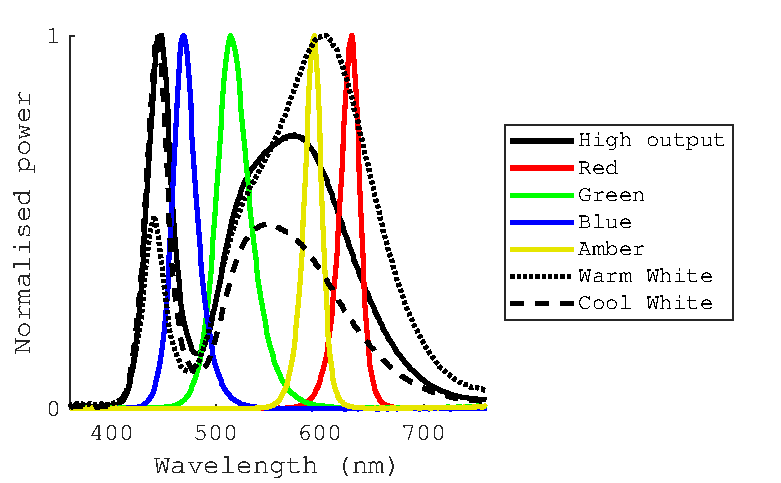
\includegraphics[max width=\textwidth]{figs/tablet/PAMELA_SPD.pdf}
\caption{\gls{SPD} of the 7 different channels available in the \gls{PAMELA} lighting rig.}
\label{fig:PAMELAlights2}
\end{figure}

\begin{figure}[hbtp]
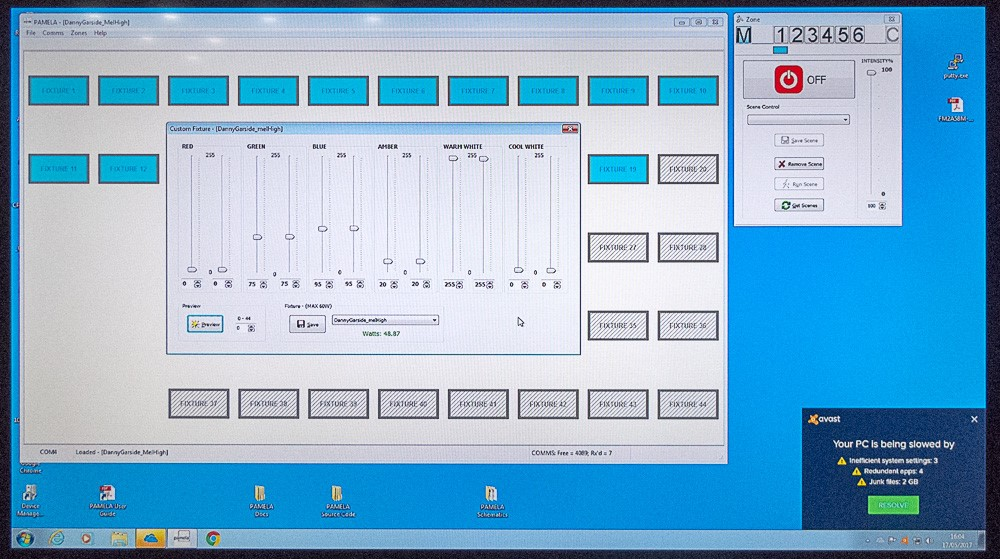
\includegraphics[max width=\textwidth]{figs/tablet/PAMELA_screenshot.jpg}
\caption{The control panel for the LED rig at \gls{PAMELA}.}
\label{fig:PAMELAlights4}
\end{figure}

For experiments reported here three illumination settings were defined - `Cool White (`CW')', `Warm White (`WW')', and `Mel-High (`MH')'. \gls{SPD}s are shown for each in Figure \ref{fig:PAMELAlights5}, and chromaticities in \ref{fig:PAMELAlights6}. `CW' and `WW' were system defaults, and `MH' was defined to be a colorimetric match (for the CIE 1931 observer) for `CW', but preferentially using an \gls{LED} band with a peak spectrally close to the peak spectral sensitivity of melanopsin ($\sim$480nm).

\begin{figure}[hbtp] %https://github.com/da5nsy/SAPS/tree/master/data/PAMELA/20180205%20Spectra
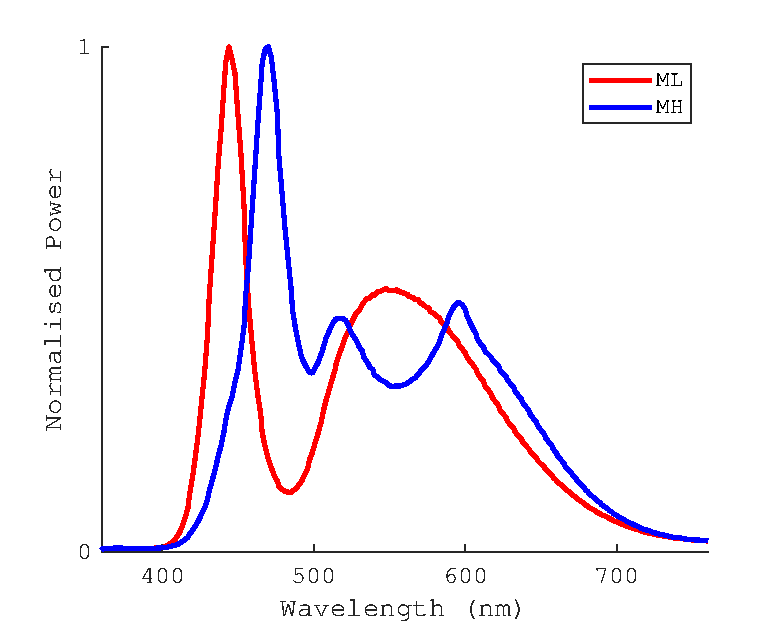
\includegraphics[max width=\textwidth]{figs/tablet/PAMELA_SPD2.pdf}
\caption{\gls{SPD}s for the colorimetrically matched illumination settings (`CW' aka `ML', and `MH') at \gls{PAMELA}.}
\label{fig:PAMELAlights5}
\end{figure}

It should be noted that luminance was not matched between the conditions. Therefore, `CW' and `MH' could be described as colorimetric matches, but not as metameric matches. Additionally, for chromatically distinct conditions (`CW' vs `WW'), there is a confound of luminance variation. The illuminances of the three conditions, measured on a horizontal plane in the centre of the experimental space, were 235lx, 689lx and 806lx for `WW', `CW' and `MH' respectively. In the opinion of the author, it would be advisable that if further studies of this type were undertaken, that conditions be matched for luminance in order to discount this as a variable. 

The chromaticities of the light sources, measured with a UPRtek MK350 (a handheld spectrometer), were:
`WW': 	u'v'(0.248,0.524) (averaged over 4 measurements);
`CW': 	u'v'(0.200,0.465) (averaged over 3 measurements);
`MH': 	u'v'(0.201,0.467) (averaged over 8 measurements).

\begin{figure}[hbtp]
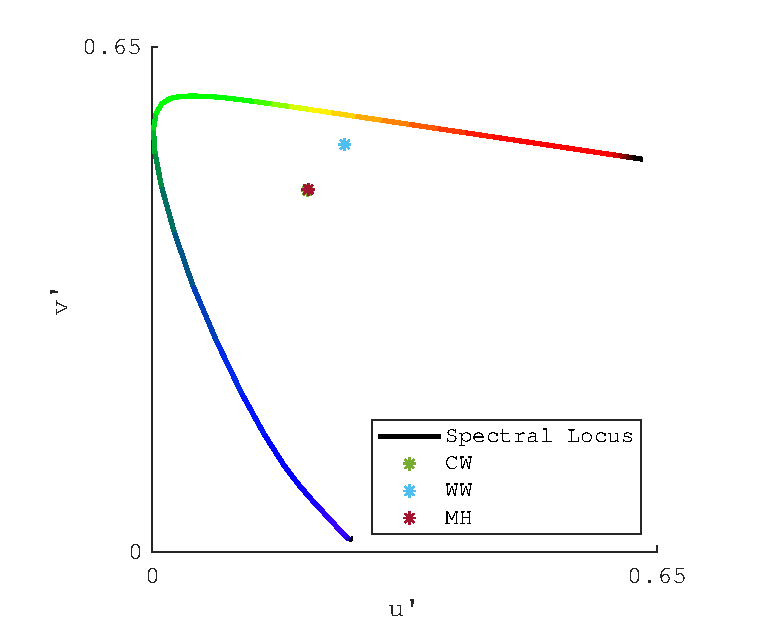
\includegraphics[max width=\textwidth]{figs/tablet/PAMELA_chromaticities.pdf}
\caption{Chromaticities of defined lighting conditions at \gls{PAMELA}. Note that `CW' and `MH' overlap.}
\label{fig:PAMELAlights6}
\end{figure}

\subsubsection{The British Museum} \label{sec:BM}

The British Museum (used for Experiment 2) is a large museum located close to the main \gls{UCL} campus, which exhibits artefacts of artistic, cultural and historical relevance. It is one of the UK's most visited tourist attractions, drawing over 5 million visitors yearly \citep{simon_calder_tate_2019}.

\medskip \noindent
Three spaces within the museum were used (with permission):

\begin{itemize}
    \item Rooms 77/78 (`Greek and Roman Architecture', `Classical Inscriptions'), lit with fluorescent lighting (CCT = 2820K SD = 31, 83 lux SD = 4, \gls{CIE}~R\textsubscript{a} = 90 SD = 0).
    \item Room 25 (`Africa' - specifically the east section of the room), lit with incandescent lighting (CCT = 2509K SD = 42, 149 lux SD = 83, \gls{CIE}~R\textsubscript{a} = 99 SD = 1).
    \item The Queen Elizabeth II Great Court (referred to as `GC'), lit with filtered daylight \citep{foster_and_partners_london._great_2002} (CCT = 6145K SD = 73, 7913 lux SD = 1891, \gls{CIE}~R\textsubscript{a} = 83 SD = 0) during daylight hours, with additional lighting at twilight and after sunset. All experiments were carried out during daylight hours.
\end{itemize}

\begin{figure}[hbtp]
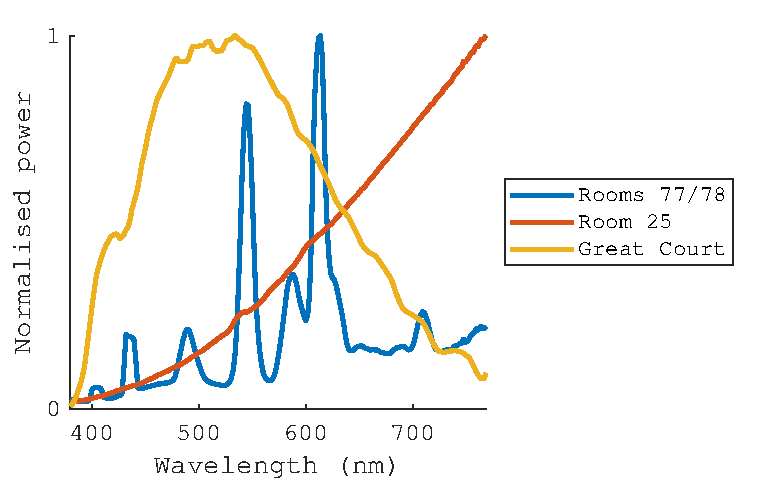
\includegraphics[max width=\textwidth]{figs/tablet/BM_SPD.pdf}
\caption{\gls{SPD}s for the environments used at the British Museum, measured with a `GL SPECTIS 1.0 touch'} 
\label{fig:BM_SPD}
\end{figure}

\begin{figure}[hbtp]
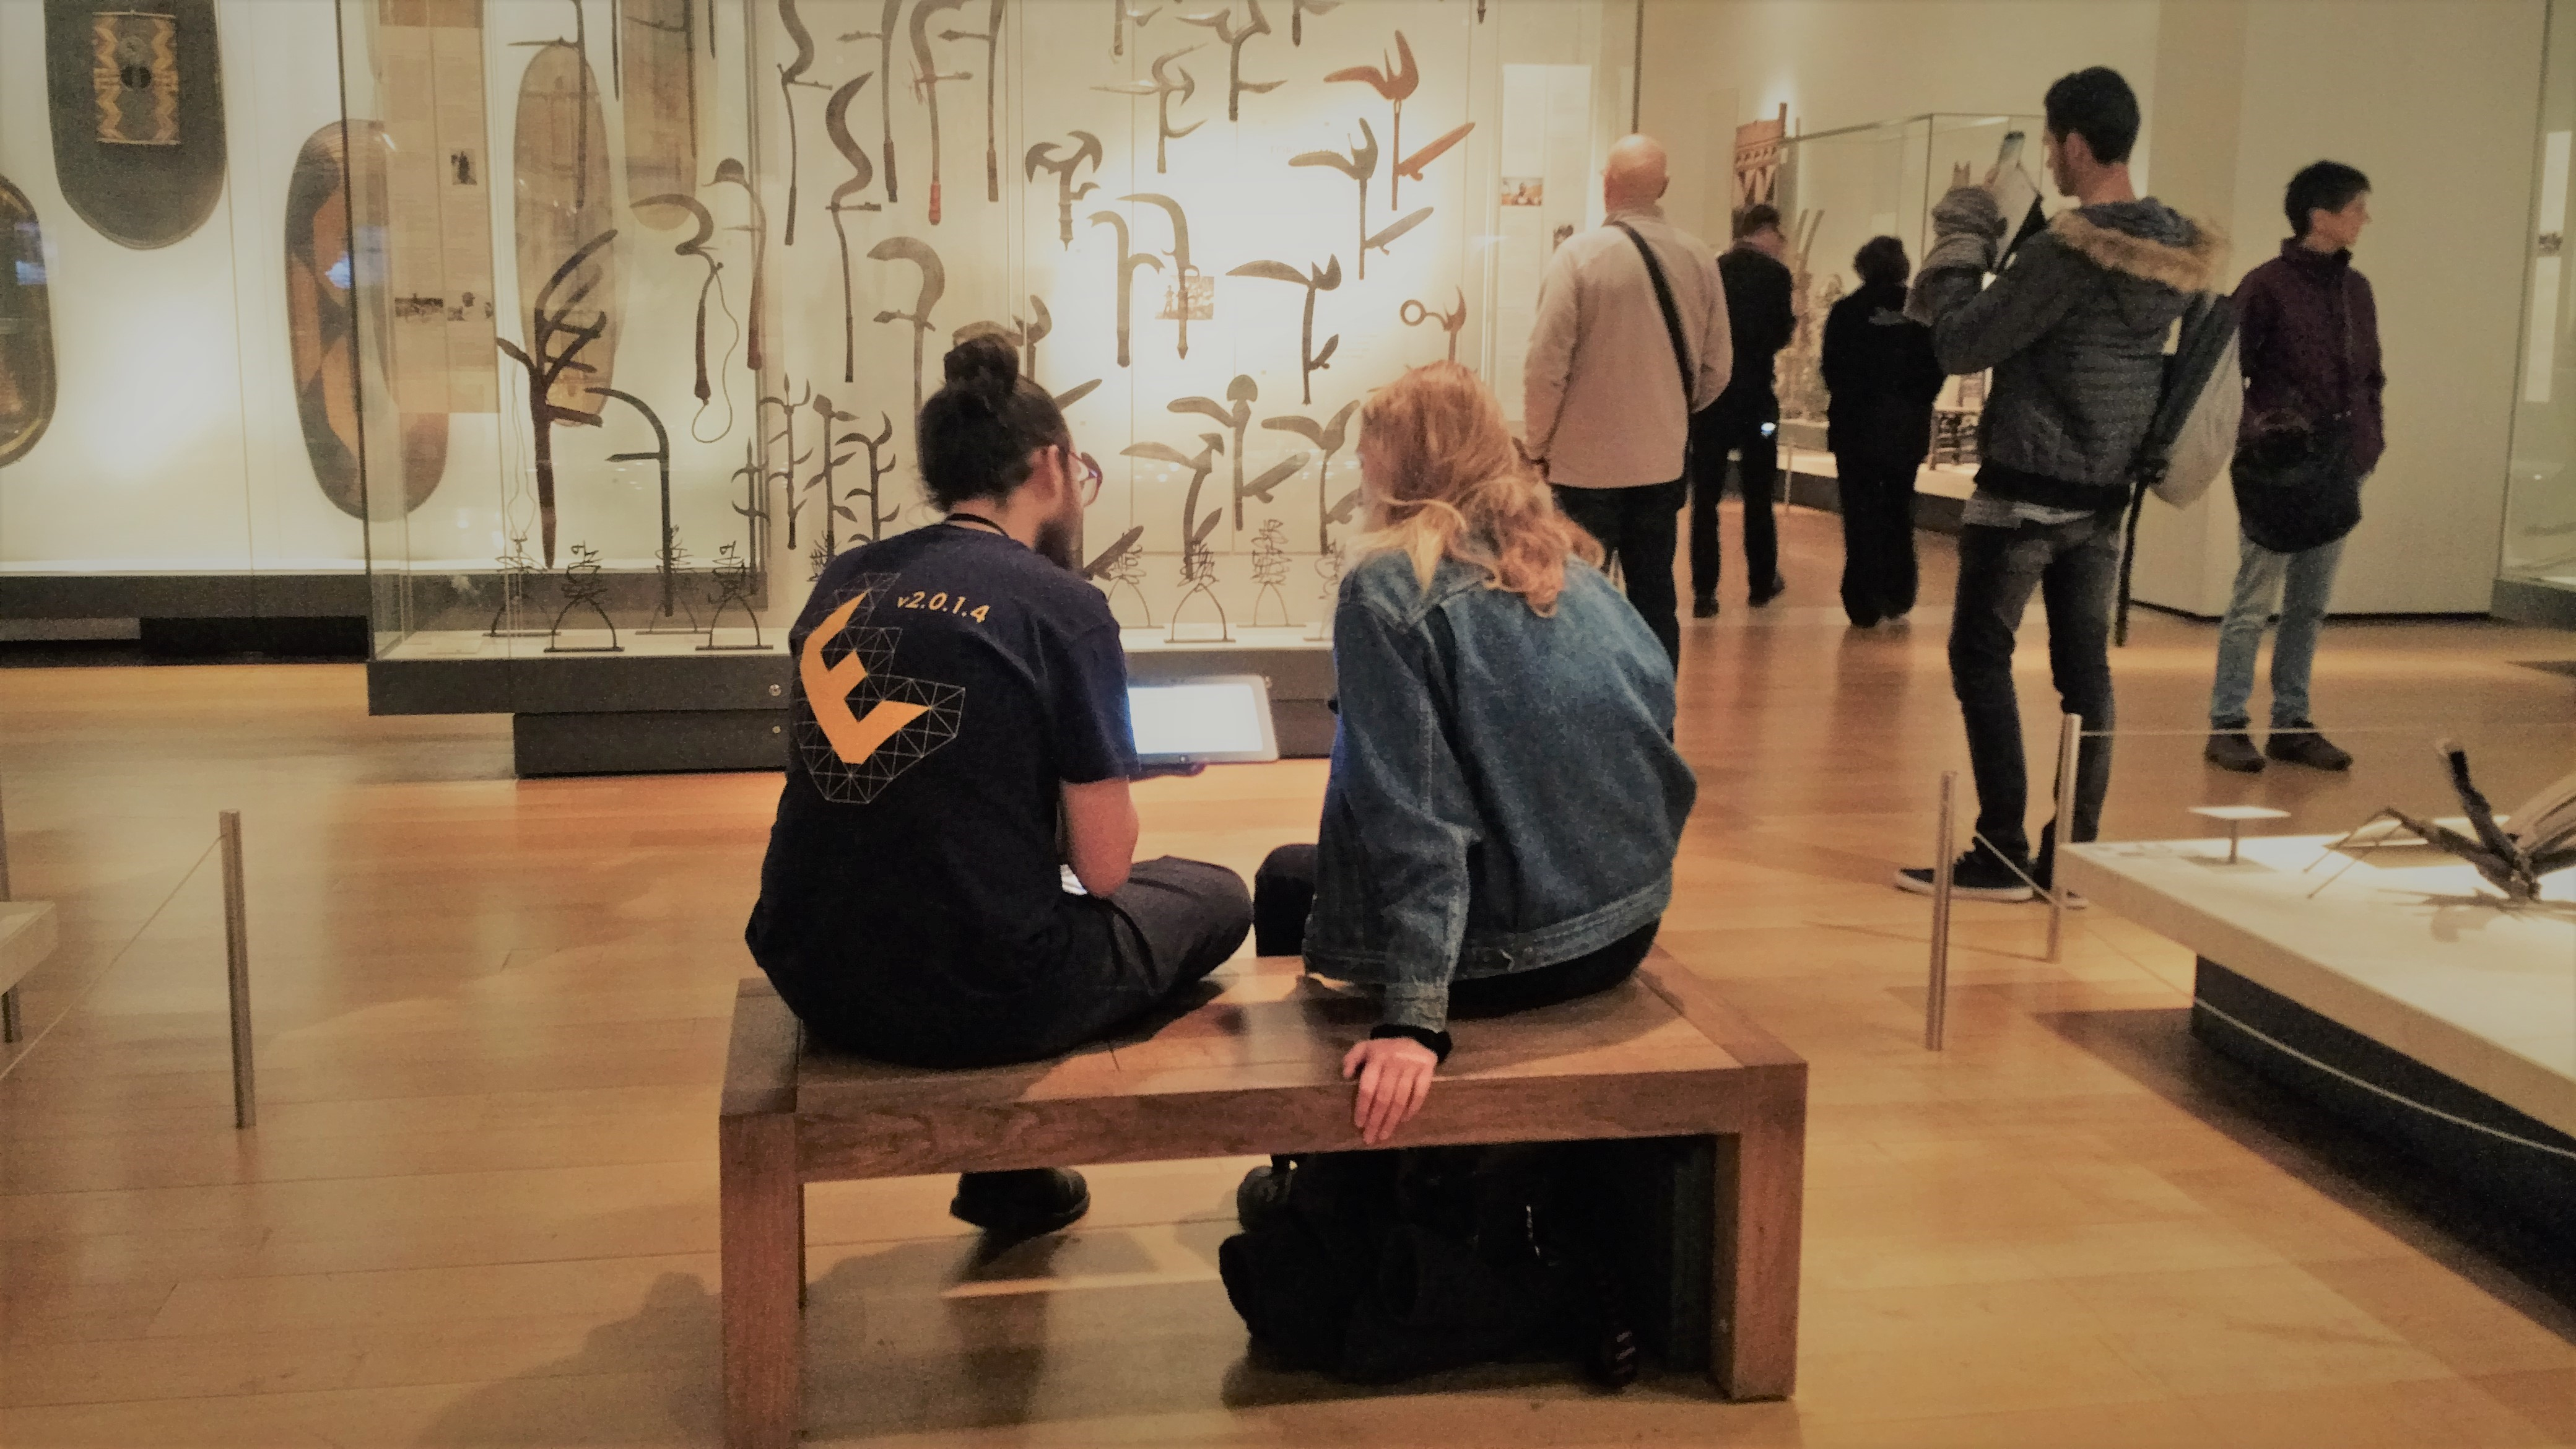
\includegraphics[max width=\textwidth]{figs/tablet/BM_Africa.jpg}
\caption{Photo of the author explaining the experiment to an observer at the British Museum. Permission to reproduce image gained from the member of public. Photo credit: Mona Hess.}
\label{fig:BM_Africa}
\end{figure}

\begin{figure}[hbtp]
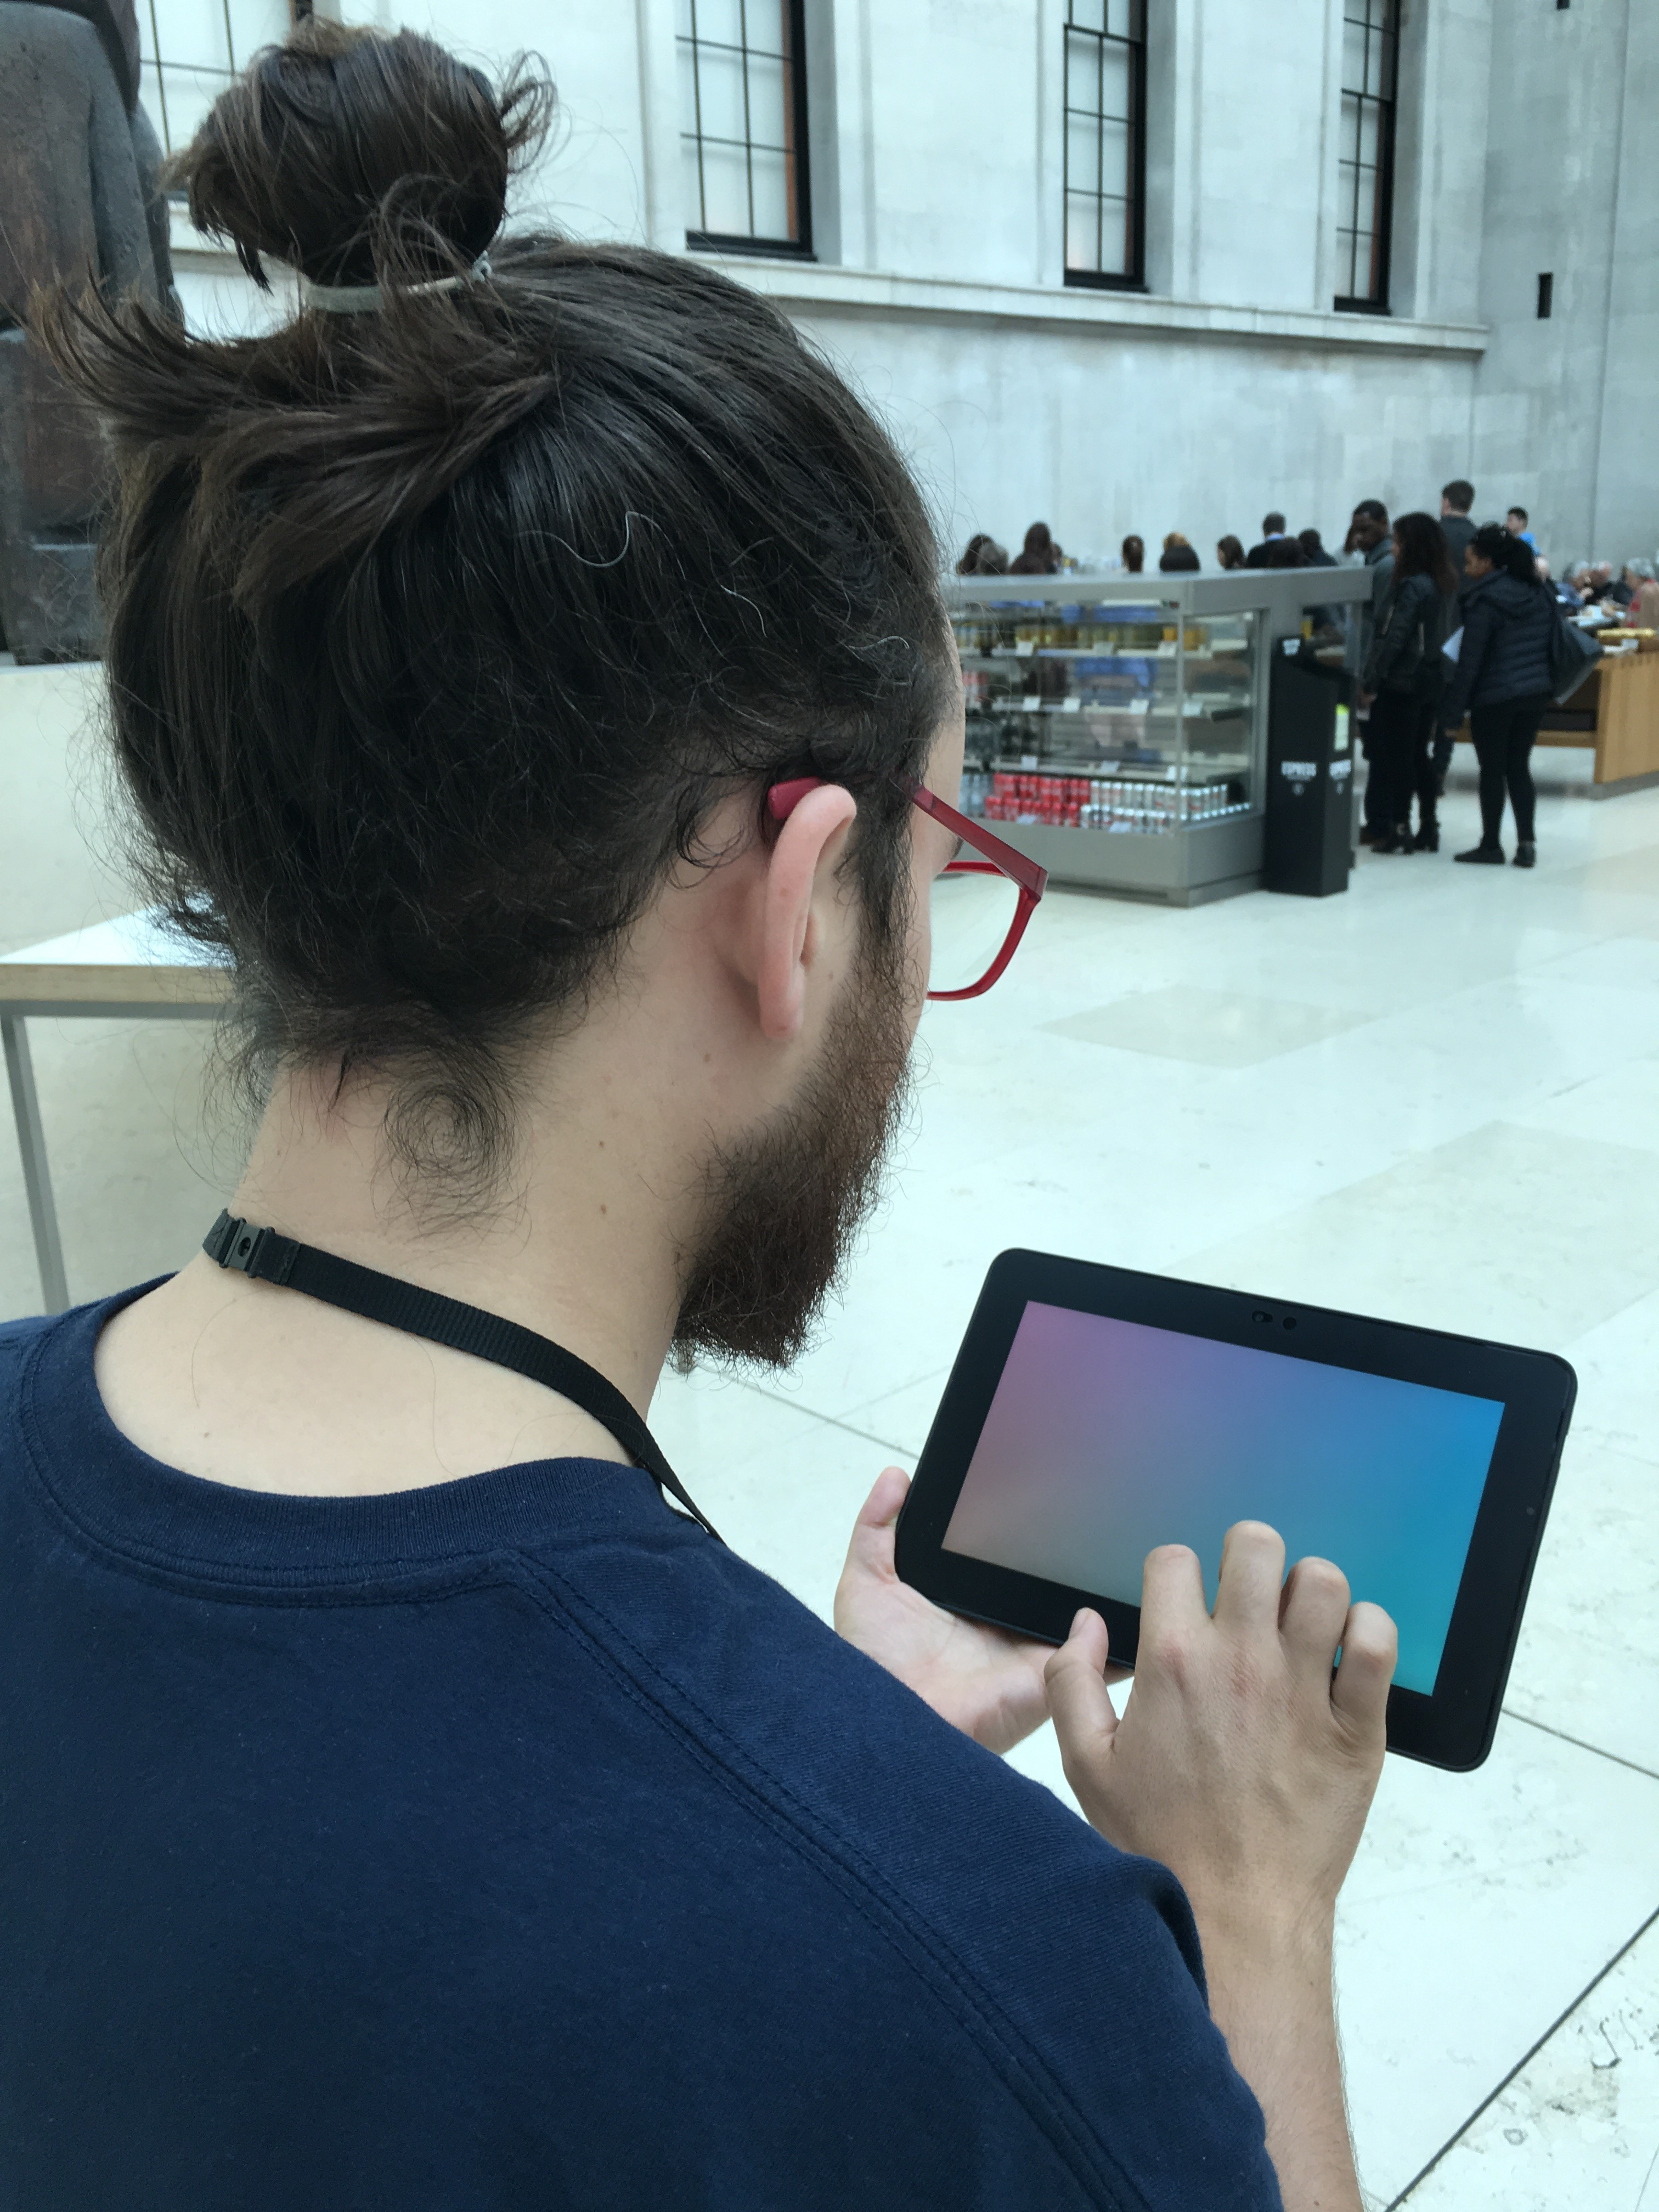
\includegraphics[max width=\textwidth,max height=0.7\textwidth]{figs/tablet/BM_GC.jpg}
\caption{Photo of the author performing the experiment in GC. Photo credit: Lindsay MacDonald.}
\label{fig:BM_GC}
\end{figure}

\begin{figure}[hbtp]
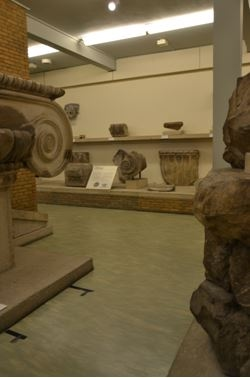
\includegraphics[max width=\textwidth,max height=0.7\textwidth]{figs/tablet/BM77.jpg}
\caption{Gallery 77, with fluorescent tube illumination. \\ Photo credit: \url{https://sites.google.com/site/jwmuseumbibletours/all-artefacts/037-temple-of-artemis-at-ephesus}}
\label{fig:BM77}
\end{figure}

These three galleries are lit with different lighting technologies of distinct chromaticities, though Room 77/78 and Room 25 are both strongly yellow, as shown in Figure \ref{fig:BMchromaticities}.

\begin{figure}[hbtp]
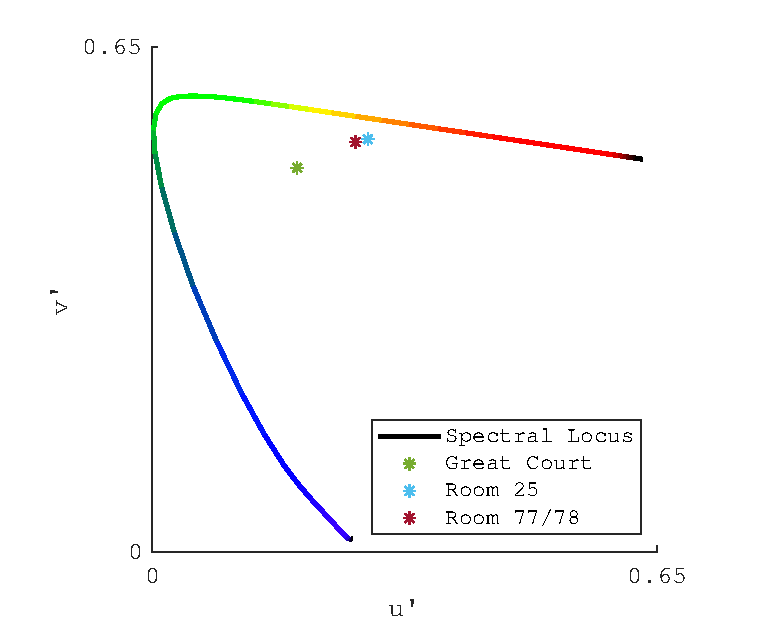
\includegraphics[max width=\textwidth]{figs/tablet/BM_chromaticities.pdf}
\caption{Chromaticities of lighting conditions at The British Museum.}
\label{fig:BMchromaticities}
\end{figure}

\subsubsection{UCL Chadwick Building} \label{sec:Chadwick}

Additional testing was undertaken within the Chadwick Building of \gls{UCL} (home of the Department of Civil, Environmental and Geomatic Engineering), in light-tight basement rooms fitted with fluorescent lighting.

% \subsubsection{\gls{UCL} Grant Museum of Zoology}

% The \gls{UCL} Grant Museum of Zoology is a natural history museum within \gls{UCL} with over 68,000 specimens, which is open to the public and also used as a teaching resource. It is lit with a mixture of daylight and \gls{LED} lighting, and a rarely used fluorescent lighting system (not used during any experiments).
% This space was used for preliminary experiments. 

% \begin{figure}[hbtp]
% 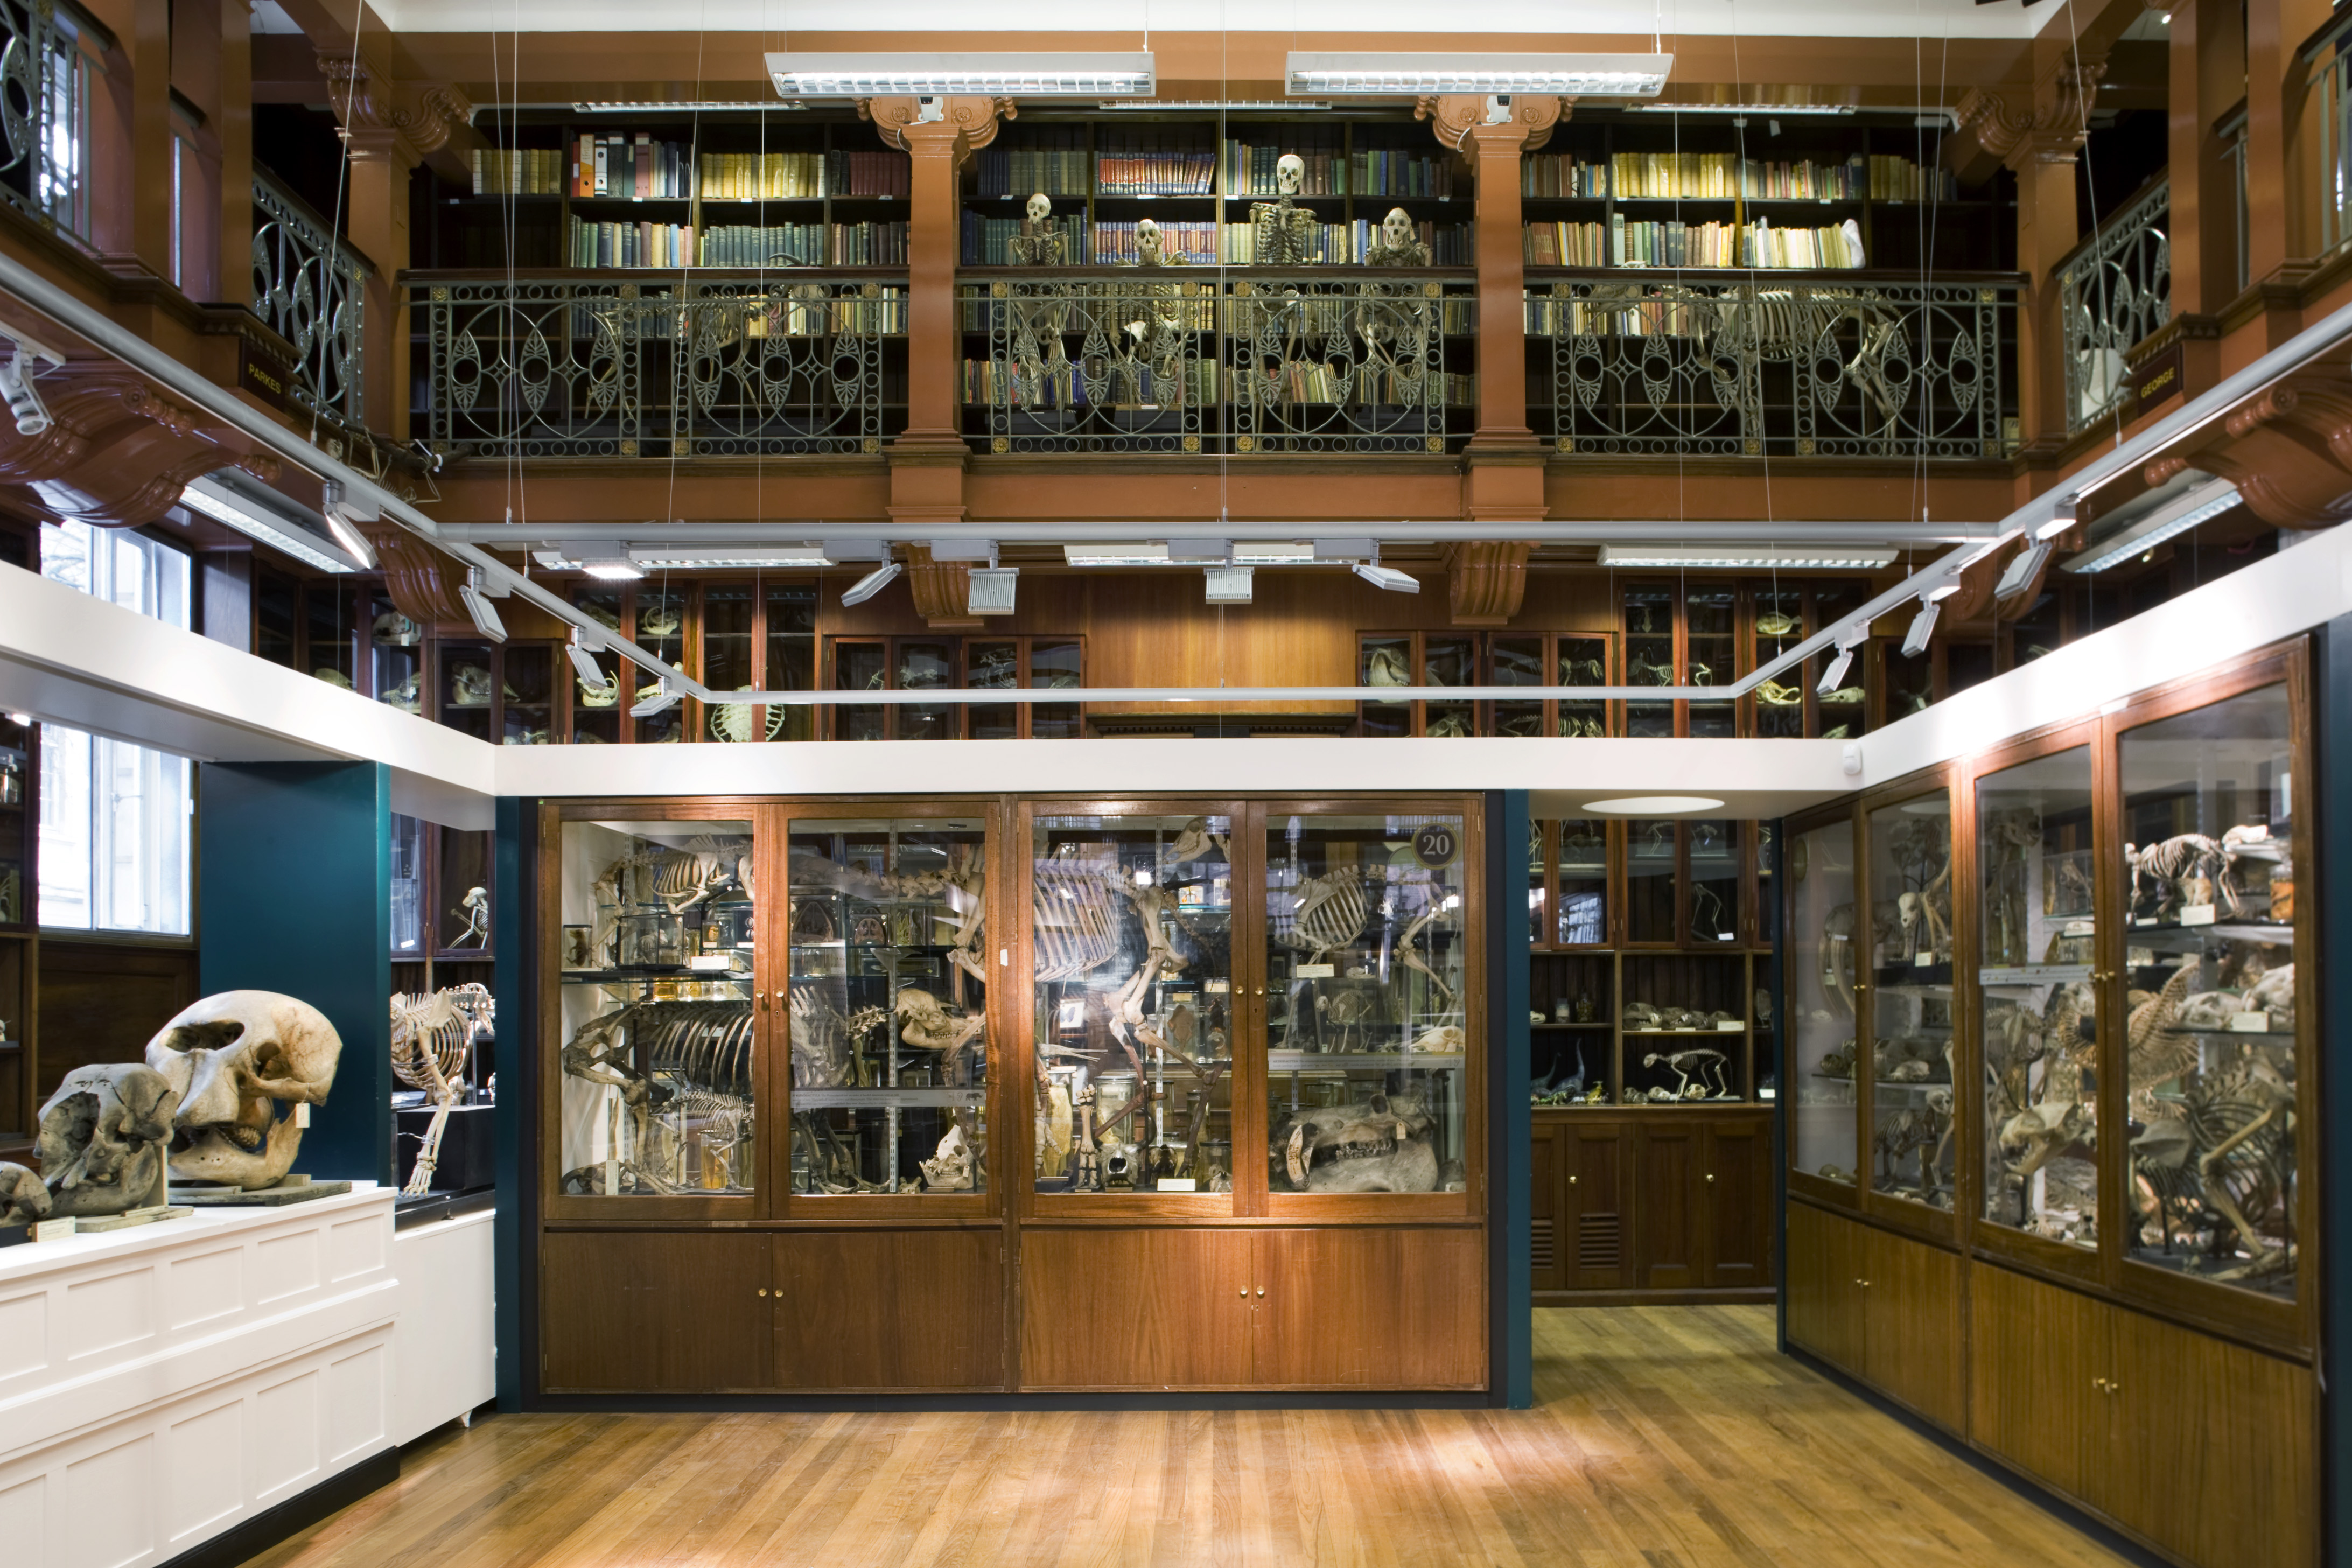
\includegraphics[max width=\textwidth]{figs/tablet/grant.jpg} 
% \caption{The central space at the \gls{UCL} Grant Museum of Zoology. Note the daylight on the left, the \gls{LED} lighting at mid-height and the fluorescent lighting at the very top of the image. Image copyright: \gls{UCL} and Matt Clayton.}
% \label{fig:grant}
% \end{figure}

\clearpage

\section{Experiments} \label{sec:SAPS_exp}

\subsection{Experiment 1} \label{sec:SAPS_exp1}
With the goal of understanding both the intra/inter-observer variability and intra/inter-environment variability, 13 runs of the experiment were performed by the author under the 3 illumination settings defined at \gls{PAMELA} (see Section \ref{sec:PAMELA}), 4 under `WW', 6 under `CW', 3 under `MH', after 2 different lengths of adaptation (5 minutes and 30 minutes). In initial analyses no effect of length of adaptation was found% write about this
, and so we group the data across these 2 conditions for analysis. Two other observers (KC and TS) also performed a number of observation (3 and 4 respectively) under a range of illumination settings.

\subsection{Experiment 2} \label{sec:SAPS_exp2}

Extending the above experiment, particularly to the inclusion of naive observers, an experiment with 58 observers was performed at \hyperref[sec:BM]{The British Museum}. See Figures \ref{fig:BM_Africa} and \ref{fig:BM_GC}.
The experiment was performed over five days, during which participants made observations in one of three gallery spaces. The three galleries used were Room 77/78, Room 25 and The Queen Elizabeth II Great Court, as described in section \ref{sec:BM}. 

\subsection{Experiment 3} \label{sec:SAPS_exp3}

In order to provide a case study for this methodology, and to investigate the role of melanopic activation upon achromatic settings, an experiment was performed at \gls{PAMELA} (see Section \ref{sec:PAMELA} for details), under the 2 of the 3 lighting conditions previously defined (`CW' and `MH'), with a repeat of `MH'. A reminder: these two lighting conditions were specified to be colorimetrically matched for the CIE 1931 observer, but with differing melanopic flux. In this experiment, the condition previously referred to as `CW' shall be referred to as with `ML' (for `mel-low'), for clarity in order to align with current literature.

The null hypothesis for this experiment is: achromatic settings are determined solely by retinal cone catches. A corollary of this is that melanopic flux plays no role. CIE 1931 chromaticity is used as a proxy for retinal cone catches.

\begin{table}[hbtp]

\begin{tabular}{|p{0.3\textwidth}|p{0.3\textwidth}|p{0.3\textwidth}|}
\hline
 & \emph{`ML' (`CW')} & \emph{`MH'} \\ \hline
Photopic lux & 689.14 & 806.25 (117.0\% of ML) \\ \hline
Melanopic lux & 694.53 & 1207.61 (173.9\% of ML) \\ \hline
CIE 1931 x & 0.312 & 0.315 \\ \hline
CIE 1931 y & 0.324 & 0.324 \\ \hline
CIE 1964 (10$^{\circ}$) x & 0.318 & 0.317 \\ \hline
CIE 1964 (10$^{\circ}$) y & 0.317 & 0.337 \\ \hline
CIE u' & 0.200 & 0.201 \\ \hline
CIE v' & 0.465 & 0.466 \\ \hline
\end{tabular}
\caption{Specifications of lighting at \gls{PAMELA}.}
\label{tab:PAMELAspecs}
\end{table}

After entering the main space at \gls{PAMELA}, the space being illuminated solely by the \gls{LED} rig in `MH' mode, and after a minimal adaptation period (5 minutes) during which introductions and instructions were given, individually performed the experimental task in succession. 

\begin{figure}[p]
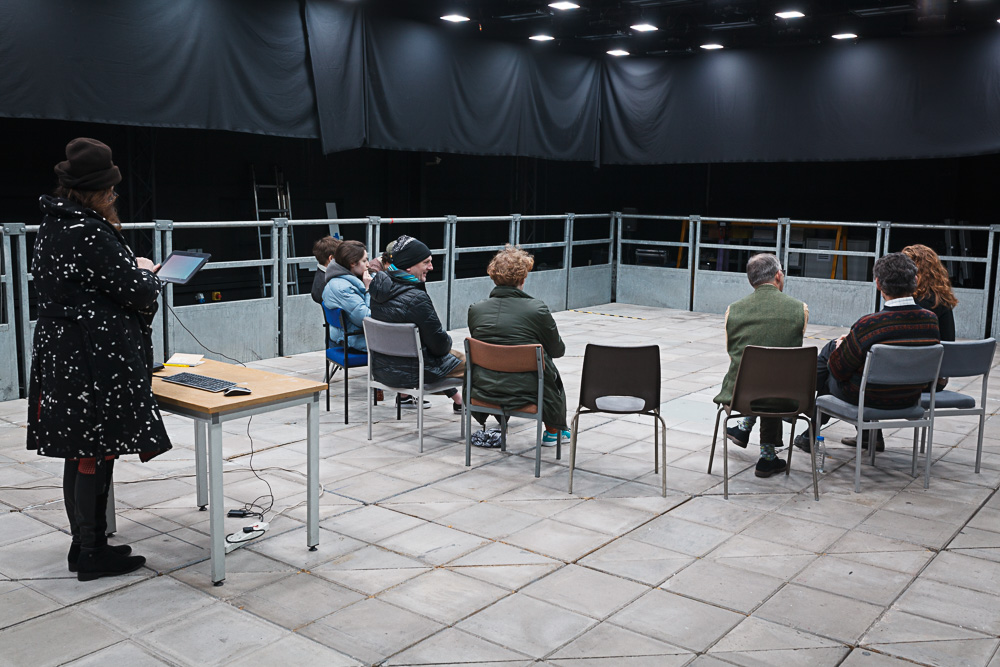
\includegraphics[max width=\textwidth]{figs/tablet/PAMELAobs1.jpg} 
\caption{The experimental set-up at \acrshort{PAMELA}. Left: an observer performs the experiment. Right: other observers wait for their turn to perform the task.}
\label{fig:PAMELAobs1}
\end{figure}

\begin{figure}[p]
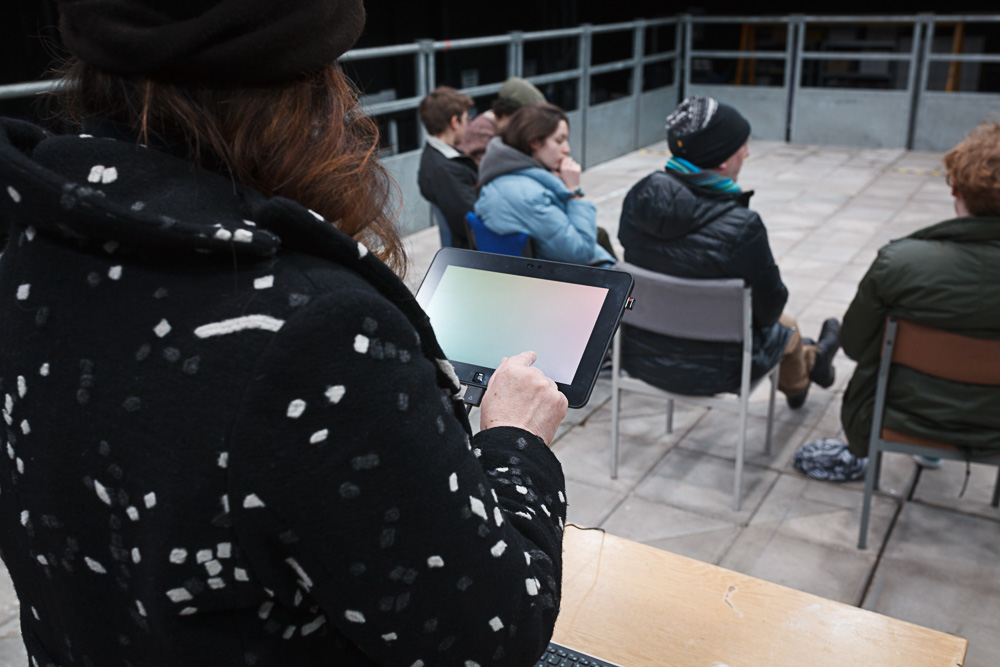
\includegraphics[max width=\textwidth]{figs/tablet/PAMELAobs2.jpg} 
\caption{The experimental set-up at \gls{PAMELA}. An over the shoulder shot of an observer performing the task.}
\label{fig:PAMELAobs2}
\end{figure}

Once each observer had performed the task once, the lighting was changed to `ML' lighting condition, and the observers again performed the task in succession. Finally, the lighting condition was returned to the initial state (`MH', referred to from now on as `MH2' to indicate that it is a repeated measure) and participants once again performed the task. Information about the nature of the lighting conditions was not provided to participants, though the change was noticeable, and observers were not informed that the third condition was a repeat of the first condition. 

When not performing the task, other participants were seated facing away from the participant currently performing the task, so as not to put pressure on the participant performing the task, and to ensure that observers were not influenced by the tactics or choices of other participants. Participants were instructed not to use phones or other electronic or light emitting devices for the duration of the experiment, but were encouraged to engage in discussion with other participants. The order in which participants performed the task was decided by the author, in an arbitrary but not properly random manner. This order was then maintained for each set of observations (the observer who performed the task first under the first condition also performed first under the second and third conditions, etc.).

Participants were not tested for colour-anomalous vision since it was shown during pilot experiments that the task itself acted as a seemingly effective colour vision test; those with colour anomalous vision struggled with the task and their data was noticeably different to data from `normal' observers. Further work is required to assess the impact of colour anomalous vision in participants when using a method such as this. 

The entire experiment took roughly 2 hours, with individual participants taking on average roughly 4 minutes to perform a single run of the experiment. This was in line with previous experience.

% The primary data collected was the spatial selections made by observers. For each observer, this amounted to 30 2-dimensional selection locations, followed by 10 calibration values. Over 9 observers, and 3 runs (`MH', `ML', `MH2'), a total of 1080 data points (where each datapoint consists of an x-coordinate and a y-coordinate) were collected (40 * 9 * 3 = 1080). Secondary data consisted of: the attributes of the stimulus on each presentation, the time taken between individual selections, an identifier for each participant, and the handed-ness of each observer.

\section{Results}

\subsection{Experiment 1}

Following data processing as described in Section \ref{sec:processing} (with no exclusions applied), a summary of data for an individual (the author) is displayed in Figure \ref{fig:PAMELA_DG_results}. 

The primary result here is that there does seem to be a distinction between the results from `WW' and the other two conditions, with the results for `WW' being displaced northeast from those for `CW' and `MH'. The means for the `WW' group and either the `CW' or `MH' groups seem to be offset by roughly 0.01 $\Delta$u'v'. If there were an effect of the ambient illumination, such as discussed in \ref{sec:ambient} this would move the recorded points in the opposite direction to that observed.

A secondary result concerns the intra-observer variability. It can be seen in \ref{fig:PAMELA_DG_results_ellipses} that the standard deviation ellipses are large, but notably smaller than the baseline data set, suggesting that the observer was actually making conscious selections. It can also be seen that there is a reliable trend of the orientation of the ellipse, which could point to an elongation along the caerulean line as seen by other researchers \citep{bosten_what_2015}. %add link to lit review

\begin{figure}[hbtp] %SAPS_DataAnalysis.m with location as 'PAMELA' and OM = 0
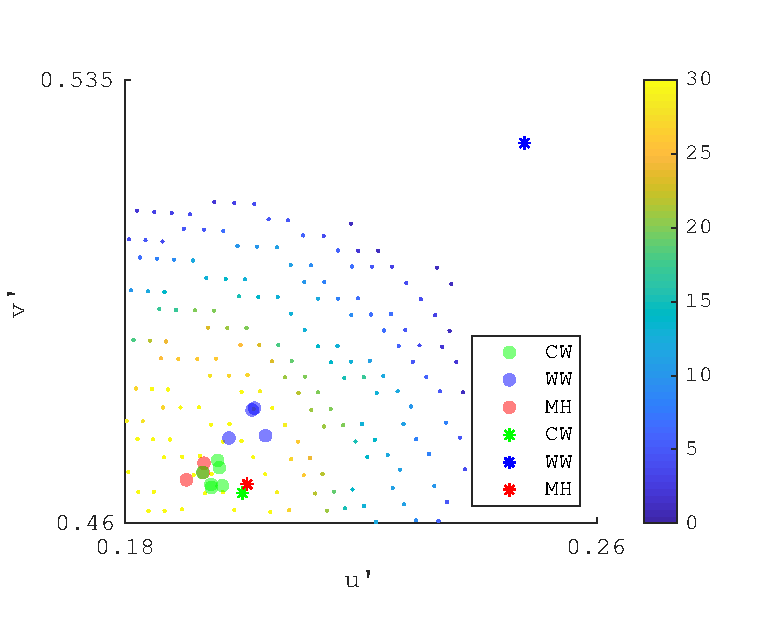
\includegraphics[max width=\textwidth]{figs/tablet/PAMELA_DG_results.pdf} 
\caption{Results for observer DG for Experiment 1. Background dots are subsampled from the practical gamut, to indicate ability of the observer to select specific chromaticities, as shown in Figure \ref{fig:practical}. Translucent red, green and blue circles represent mean chromaticity selections per run. Red, green and blue asterisks represent illuminant chromaticities for different conditions.}
\label{fig:PAMELA_DG_results}
\end{figure}

It can be seen in Figure \ref{fig:PAMELA_DG_results} that the chromaticity of the `WW' illuminant falls far outside the practical gamut; there would have been no opportunity throughout the entire set of runs where the observer would have been able to select a pixel of a chromaticity matching that illuminant. It might therefore be expected that we would see an extended smearing pattern in selections away from the centre of the practical gamut towards the chromaticity of this illuminant, as discussed in Section \ref{sec:limitations}. This effect is indeed visible, see the extended nature of the blue ellipses in Figure \ref{fig:PAMELA_DG_results_ellipses}.

\begin{figure}[hbtp] %SAPS_DataAnalysis.m with location as 'PAMELA' and OM = 1
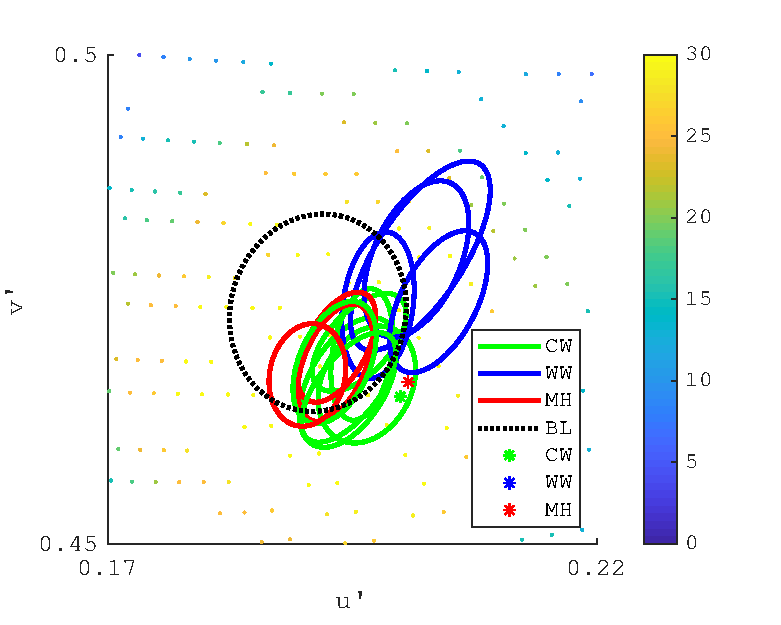
\includegraphics[max width=\textwidth]{figs/tablet/PAMELA_DG_results_ellipses.pdf} 
\caption{As per Figure \ref{fig:PAMELA_DG_results}, but re-scaled and showing standard deviation ellipses to indicate spread of data. `BL' is a baseline dataset, representing an observer hitting the spatial centre of the screen for every stimulus. It can be seen that in comparison to this baseline, there is a trend whereby selections are elongated along the positive diagonal. The results for `WW' seem particularly elongated along this axis, which I assume to be the result of the chromaticity of `WW' laying outside of the practical gamut.}
\label{fig:PAMELA_DG_results_ellipses}
\end{figure}

% KC and Tatsuto? %!!!!!!!!!!!!!

\clearpage

\subsection{Experiment 2}

\subsubsection{Exclusions}

Considering that this experiment was performed with observers selected from the general public it seems reasonable to assume that we may need to use exclusion criteria. Now that we have real data we can consider the two options presented in Section \ref{sec:exclusion}.

For Figure \ref{fig:excl1} `Mean SD' is calculated for each observer's data by taking the mean of the standard deviation in the u' and v' chromatic dimensions. \gls{DBUR} is calculated as the Euclidean distance between the two chromaticity coordinates selected for the two identical stimuli.

\begin{figure}[hbtp] 
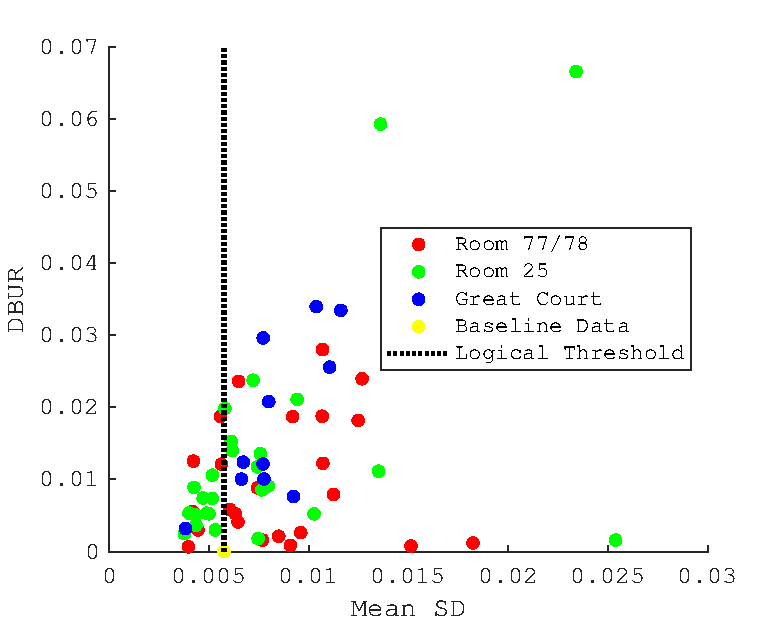
\includegraphics[max width=\textwidth]{figs/tablet/excl1.pdf} 
\caption{The two measures of variability set against each-other, for the data collected in Experiment 2.}
\label{fig:excl1}
\end{figure}

It can be seen that on both measures there are a small number of clear outliers; three points with high mean SD but low \gls{DBUR}, and two points with both high mean SD and high \gls{DBUR}. Using only one of these two measures would fail to pick up some of these points, though as a single measure mean SD seems as though it would be more effective in recognising these points.

A vertical line (the `logical threshold') is plotted from the point representing baseline data. This data is calculated by computing the results for a hypothetical observer who pressed the precise centre of the screen for each stimulus, and the precise centre of the checker-board on the touch characterisation phase. 

As can be seen from this line, a threshold based on this measure would exclude a very large number of datasets. This is partly due to the fact that most real observer's exhibit orientation-dependent variability, with the greatest axis of variability generally being in line with the caerulean line, whereas the hypothetical data is nominally rotationally symmetric (see Figure \ref{fig:PAMELA_DG_results_ellipses}). It may be more appropriate then to compare the SD of the hypothetical dataset to the SD of the axis of least variability for real data. However, this could be seen as being overly lenient towards the real data. As a compromise, and for simplicity, let's consider the minimum value between u' SD and v' SD (rather than the mean) as the representative for real data, which shifts relative positions of the data and the threshold such that more datasets pass this test. 

\begin{figure}[hbtp] 
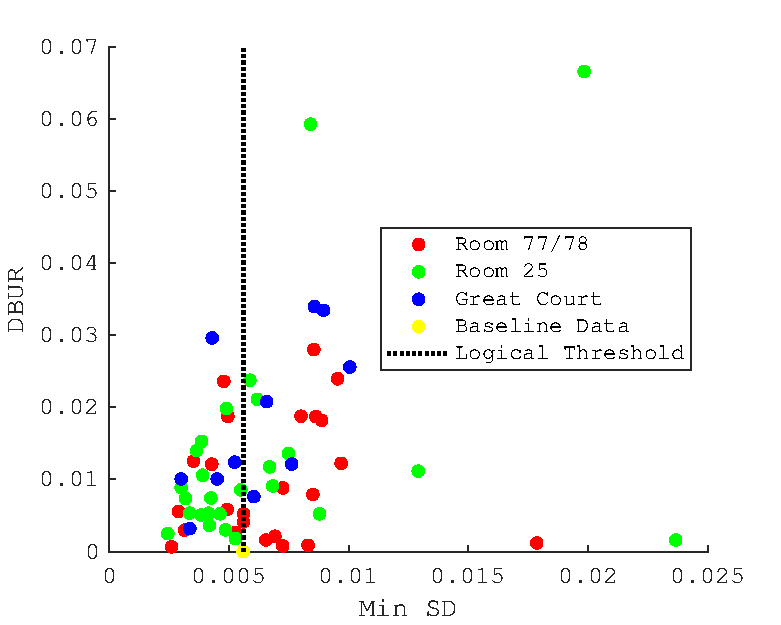
\includegraphics[max width=\textwidth]{figs/tablet/excl2.pdf} 
\caption{As \ref{fig:excl1} but with minimum standard deviation (whichever is lesser between u' and v') plotted on the x-axis rather than the mean.}
\label{fig:excl2}
\end{figure}

This test still seems rather severe (Figure \ref{fig:excl2}), and this is likely due to several issues. Firstly, the theoretical data does not have any element of variability introduced from touch uncertainty. Secondly, since the hypothetical data is firmly centred on the spatial centre of the screen it avoids any element of aforementioned `smearing' (where an observer might ideally select a point outside of the display gamut). Thirdly, in situations where there is a high variation across both the u' and v' axis, but a minimum is another dimension (in other words: strongly elliptical data orientated roughly diagonally in chromaticity space), which seems common for this type of data, the minimum between u' and v' is still going to be an overestimation of a truly representative SD.

Whilst the second measure suggests no clear rationale for a threshold boundary, there is a greater spread in the variability of these differences between observers, and the relationship between this measure and an observer's performance follows a strong and clear logic.

In the absence of a clear logical framework from which to draw a specific cut-off value for DBUR, I shall propose 0.04 which aligns with an apparent divide in this specific dataset, since there is a possibility that this divide represents a functional divide between observer behaviours. It also seems reasonable to exclude data with a Min SD \textgreater 0.01, again with the rationale that for this specific dataset points above this boundary appear to be outliers from the rest of the group. These two cut-offs, which exclude 6 observers from this data, are visualised in Figure \ref{fig:excl3}.

\begin{figure}[hbtp] 
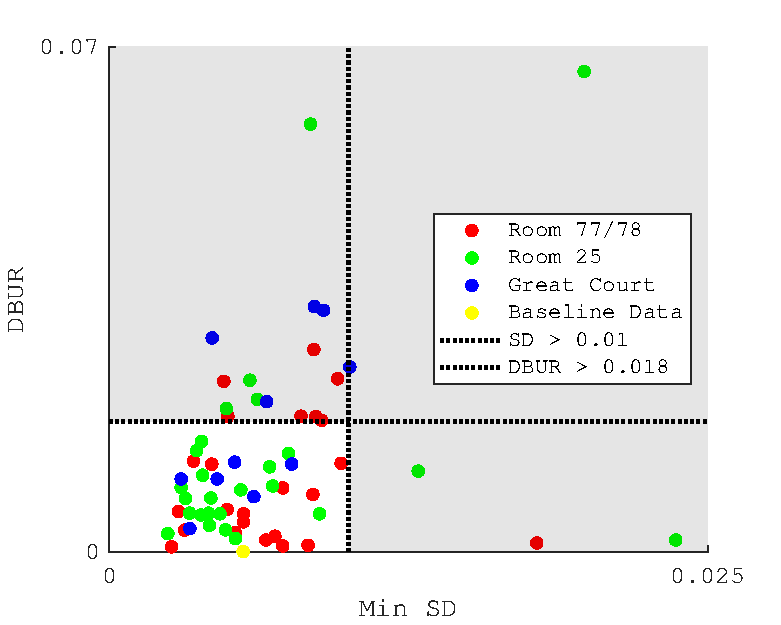
\includegraphics[max width=\textwidth]{figs/tablet/excl3.pdf} 
\caption{As \ref{fig:excl2} but with proposed boundaries}
\label{fig:excl3}
\end{figure}
% Probably could combine some of the above graphs.

\subsubsection{Data}

Data without exclusions is presented in Figure \ref{fig:exp2wo}. Following exclusions, data is presented in Figure \ref{fig:exp2}. The exclusions do not seem to target a specific type of data, nor do they seem to change any apparent trends or results for this specific dataset. Both before and after, we see a distinction between the `GC' data and the data from the other two locations, which may have been expected from the distinct chromaticity of the lighting. It is worth noting however, that luminance in this environment was generally very high, and so there is an increased risk of the stimulus deviating from the desired colorimetry (as noted at the end of Section \ref{sec:ambient}).

We see that the chromaticities of the ambient lighting in the first and second environments (77/78, and 25) are far outside the practical gamut. If we might have expected full chromatic adaptation in observers in these environments, then the results we see would represent the case where there is extreme smearing (similar to the `most yellow' dataset from Figure \ref{fig:basement_rgby_test}). 

\begin{figure}[hbtp] 
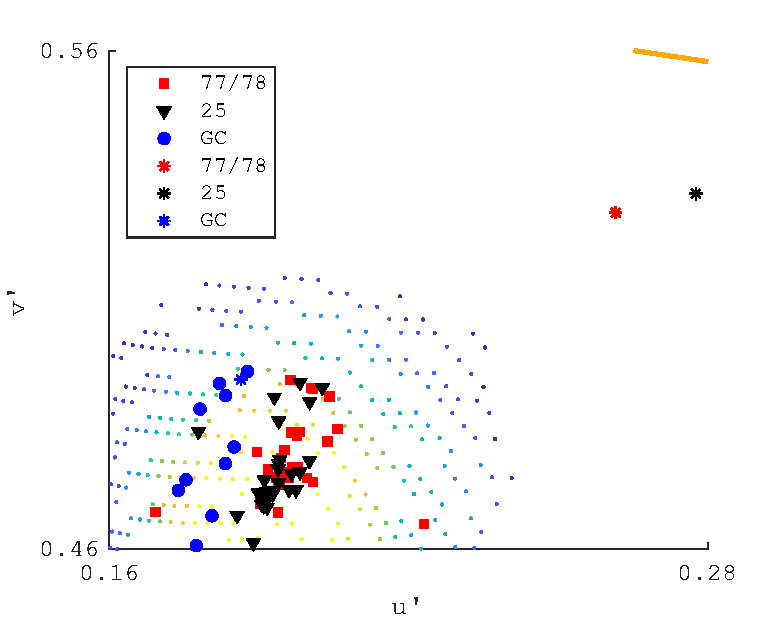
\includegraphics[max width=\textwidth]{figs/tablet/exp2_withoutExclusion.pdf} 
\caption{The mean settings of all observers from Experiment 2, with illuminant chromaticities for the 3 different spaces.}
\label{fig:exp2wo}
\end{figure}

\begin{figure}[hbtp] 
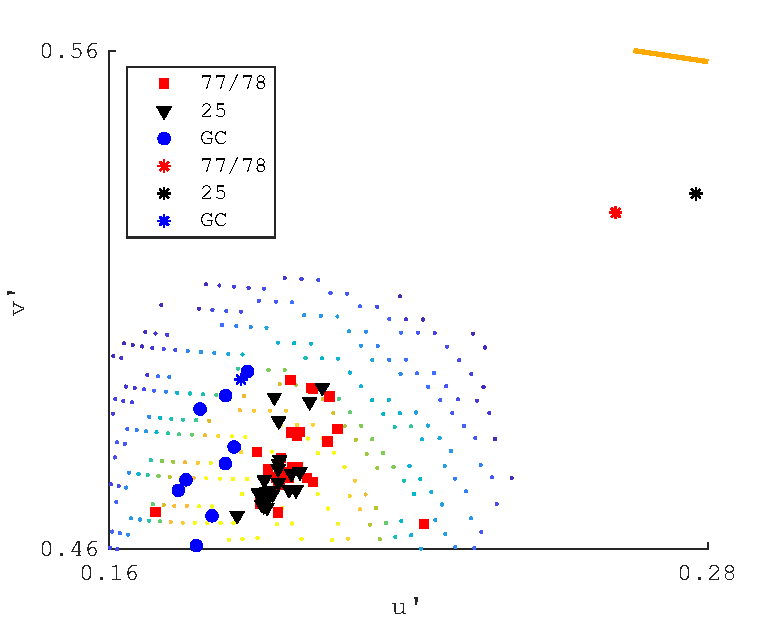
\includegraphics[max width=\textwidth]{figs/tablet/exp2.pdf} 
\caption{As \ref{fig:exp2wo} but with exclusions applied. Note the reduction in black points (Gallery 25) around [0.19,0.47], and the reduction the blue points (GC).}
\label{fig:exp2}
\end{figure}

In summary, for the data collected at the British Museum, we see a distinction between the `GC' data and the data collected in the two other environments and minimal distinction between those two other datasets. This tallies well with witnessing a distinction where lighting chromaticity is distinct, and minimal distinction where lighting chromaticities are similar. However, this method did not allow for the selection of chromaticities which would have represented a true non-spectrally-selective surface under two of these lighting conditions, and so the data for those conditions is unlikely to be a simple representation of an observer's chromatic adaptation state.

The potential confounds in this experiment are, at minimum: observer (and associated variables), day and time, gallery space, luminance, and lighting technology.

A subset of this data will be used in the \nameref{sec:tablet_Discussion} section to comment upon the applicability of this method to naive observers (Section \ref{sec:naive}).

\clearpage

\subsection{Experiment 3}

Initial exclusions were based on the criteria decided for Experiment 2 (Min SD \textgreater 0.01, \gls{DBUR} \textgreater 0.04). This is visualised in Figure \ref{fig:exp3excl}. One observer, with all points above the min SD threshold was immediately excluded. The decision was made to exclude two further participants, one where one of their runs exceeds the min SD threshold, and another who is below both thresholds but still outside of the main grouping for all three runs.

\begin{figure}[hbtp] 
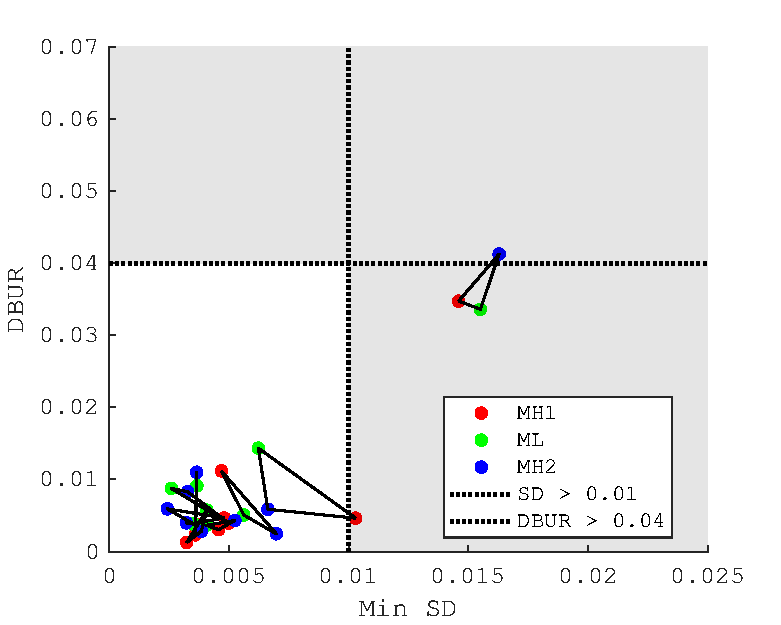
\includegraphics[max width=\textwidth]{figs/tablet/exp3excl2.pdf} 
\caption{As per Figure \ref{fig:excl3} but for Experiment 3 data. Triangles connecting points denote specific observers.}
\label{fig:exp3excl}
\end{figure}


Following exclusions, averages for the remaining dataset can be plotted, coloured for lighting condition, as shown in Figure \ref{fig:PAMELA_20180205_results}. There is no clear distinction between datasets collected under different lighting conditions.

\begin{figure}[hbtp] %https://github.com/da5nsy/SAPS/blob/bb463ae303a800c6bcadb5295fa4c9db4562499f/SAPS_DataAnalysis.m
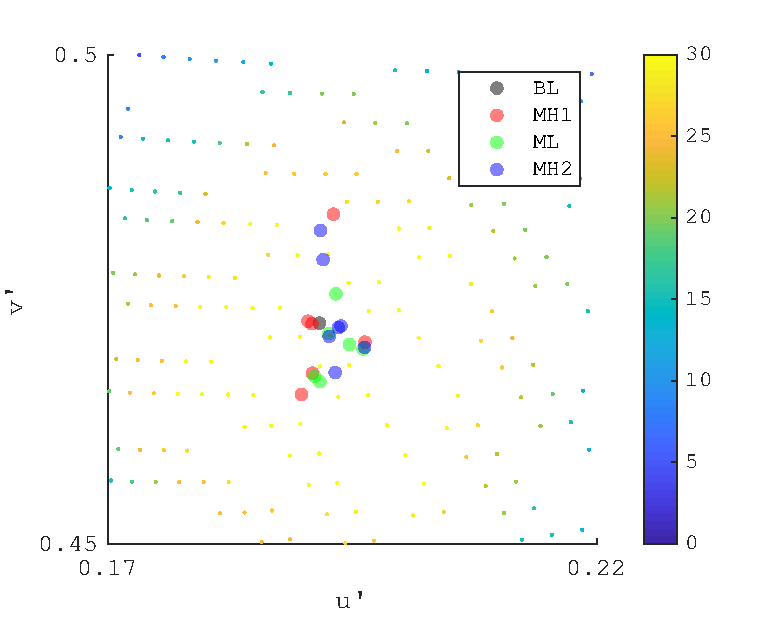
\includegraphics[max width=\textwidth]{figs/tablet/PAMELA_20180205_results.pdf} 
\caption{Results summarised as means for the 2 different lighting conditions (MH2 is a repeat of MH1).}
\label{fig:PAMELA_20180205_results}
\end{figure}

Plotting data for individual participants separately, it can be seen that each participant exhibits moderate self-correlation; in successive trials, despite changes in illumination, individuals provide data which appears to be similar across conditions, sometimes with a reliable bias per observer. See Figures \ref{fig:PAMELA_20180205_Individual} and \ref{fig:PAMELA_20180205_Individual2} for examples of data from 2 participants, noting that the black ellipse (the baseline data) is the same for both observers and can be used as a visual anchor for comparison. Between these two observers it can be seen that the first reliably chooses points with a bias towards the lower left compared to the baseline data, whereas the second has a bias towards points on the right of the baseline data. 

\begin{figure}[hbtp]
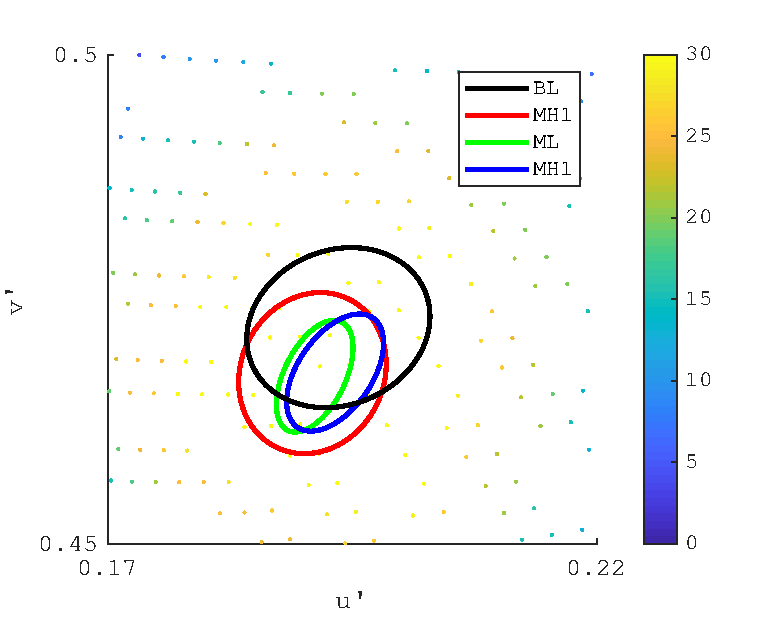
\includegraphics[max width=\textwidth]{figs/tablet/PAMELA_20180205_Individual.pdf} 
\caption{Standard deviation ellipses for observer PK.}
\label{fig:PAMELA_20180205_Individual}
\end{figure}

\begin{figure}[hbtp]
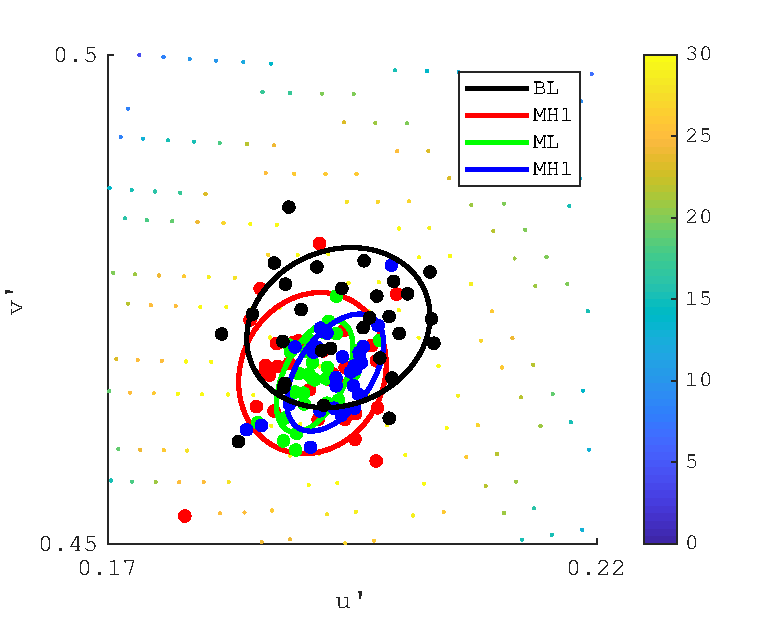
\includegraphics[max width=\textwidth]{figs/tablet/PAMELA_20180205_Individual2.pdf} 
\caption{Standard deviation ellipses for observer LM.}
\label{fig:PAMELA_20180205_Individual2}
\end{figure}

From these two figures it can be seen that, at least in this case, there is moderately large inter-observer variation. It is possible that when using a large number of observers an additional processing step may be required to offset for observer bias. In this case inter-observer variation does not seem to be masking a distinction between the conditions.

\clearpage

\section{Discussion} \label{sec:tablet_Discussion}

In the following section I shall discuss the proposed methodology in terms of its abilities and limitations, referring in turn to the hypotheses stated at the start of this chapter (Section \ref{sec:qandhyp}), and areas that I consider worthy of further consideration or development. I shall also comment on the results of Experiment 3.

\subsection{Environment-agnostic stimulus}

As discussed in Section \ref{sec:ambient}, this specific stimulus, under the lighting conditions defined at \gls{PAMELA} is only minimally affected by changes in illuminant, and that any effect would principally affect the outer edges of the stimulus space.

It is also worth noting that the effect upon collected data of an illuminant induced shift in display colorimetry, would actually be opposite to the effect that one would expect to see from a change in observer adaptation state. For example, under a hypothetical blue light, which affected the stimulus by making it more blue, an observer would be inclined to select something more towards the yellow side of objective white. 

It should be noted that this result is expected to break down under illumination at higher levels than that tested at \gls{PAMELA}.

\subsection{Meaningful data}

\subsubsection{Intra-observer Variability: Touch input}

One insight into variability within this method can be taken by looking at the calibration data that each participant provides after the main part of each trial (Described in Section \ref{sec:touch}). Here they are asked to touch the centre of a checker-board, and this data is primarily used to offset any bias introduced by the difference between where an observer thinks they are touching, and where the tablet records having been touched. A secondary use of this data, albeit with caveats, is to estimate the amount of variation introduced simply by touch imprecision; here the participant is given as-close-to an objective task as might be thought possible, and thus any variability in the results must stem not from perceptual indecision, but rather the process of pointing and touching. There is a clear caveat; it seems likely that an estimate of touch imprecision gleaned from this dataset will underestimate the amount of `real' touch imprecision, since observers have reliably (in my experience) modified their touching behaviour in this second part of the task, in the manner which might be expected of someone who is given a broad target to hit, and then immediately after is given a much smaller target to hit (they lean in, hold their finger more rigidly, and move more slowly).

To perform this analysis I shall use the data from Experiment 2, to get the largest possible sample and so as not to limit the analysis to those with a strong vested interest in this research. In Figure \ref{fig:BMtouch} I show the standard deviations based on just the calibration (checker-board) data. Note that here the units are pixels, as opposed to a chromaticity space. 4 outliers are excluded. These outliers appear to occur due to an observer accidentally double-touching the screen during the calibration phrase, and thus having one data point which is far outside the normal group. This does not affect (to a large extent) the actual calibration process, because there a median is taken, but it does have a rather strong effect when calculating the standard deviation of a set.

\begin{figure}[hbtp]
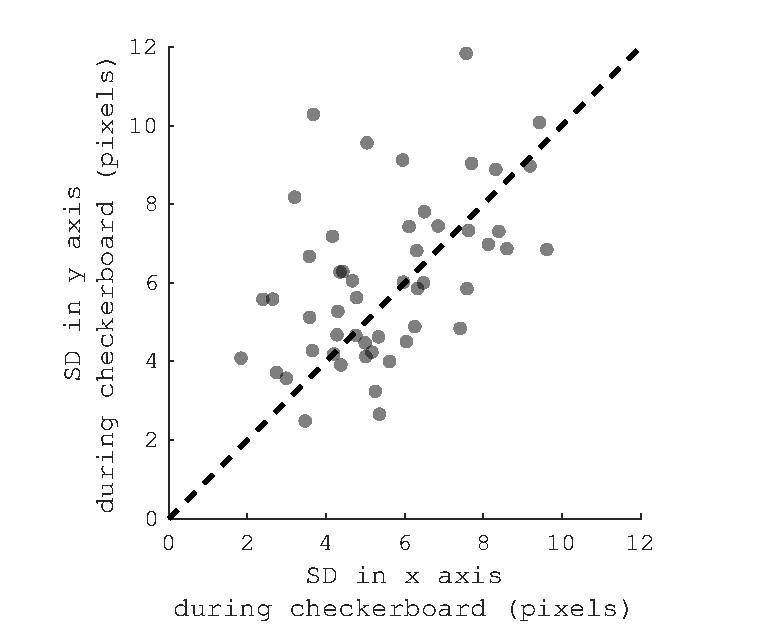
\includegraphics[max width=\textwidth]{figs/tablet/BMtouch.pdf} 
\caption{Standard deviations for the calibration datasets from the Experiment 2 data. Added for additional interest is the line of unity, which makes clearer the imbalance between SD in the x axis and the y axis - on this task an observer seems more likely to be have worse vertical discrimination. It is unclear whether this is a task specific result or a general phenomenon.}
\label{fig:BMtouch}
\end{figure}

To consider the above information in practice, we need to perform a conversion into chromaticity space. For a simple analogy, let's consider a pixel shift of 6 pixels (the rough average standard deviation in each dimension, based on a visual analysis of Figure \ref{fig:BMtouch}). Considering that the full stimulus is 2188 pixels wide, and represents u* -50:50 (100 u* units it total), a single pixel shift represents a shift of 0.0457 u* units. Converting this to u' (u' = u*/(13.L*)), gives us a value of 5.8590e-05 u' per pixel, and 3.5154e-04 u' for 6 pixels which is an order of magnitude smaller than the average standard deviations for the main datasets. I therefore conclude that touch imprecision will only have a minor influence on the data collected with this method, especially when an effort is made to calibrate out this bias. Further investigation may conclude that this element of measurement imprecision is not worth the effort required to correct for. It should be noted however, that by performing this analysis based on variance we have implicitly ignored any systemic hardware bias (say if every measurement was off by 20 pixels in the same direction, this would be corrected for in the data processing, but would not be picked up by this specific analysis.)

%% -50:50 (100 total) across 2188 pixels
%% each pixel =
%100/2188 %0.0457 u*
%% and u' = u*/(13xL*)
%% and we define L* to be 60
%% so 0.0457 u* =
%0.0457 /(13*60) % 5.8590e-05
%% so 6 pixels =
%ans * 6 %3.5154e-04 u'

\subsubsection{Intra-observer Variability: Test-retest}

Our assumption is that observers would have a reasonably stable point of adaptation during their undertaking of the experiment, and that variability in the data would primarily be due a combination of fuzzy boundary of acceptability and input imprecision. 

This variability is of particular interest because it impacts the power with which we are able to distinguish two distinct states of chromatic adaptation.

The data available with the largest number of repeats by a single observer is that of Experiment 1, as shown in Figure \ref{fig:PAMELA_DG_results_ellipses}. Here it can be seen that the standard deviation ellipses are considerably smaller than the baseline data, and that repeated measures under the same condition are reliably placed. The standard deviation of the means of runs under `CW' (where there were 6 repeats) is [u',v'] = [0.0012,0.0019]. Compared to the offset between the means between the two sets which we think to be different (`CW' vs `WW'), offset: ([$\Delta$u',$\Delta$v'] = [0.0061,0.0091]), there is shown to be roughly a factor of 5 (1./([0.0012, 0.00190]./[0.0061, 0.0091]) = [5.1, 4.8]), suggesting that if our estimate for standard deviation is correct, and if our effect size is correct and generalizable to other situations, this method should be able to reliably detect meaningful differences in response.

\subsubsection{Inter-environment Differences}

Considering the standard theories of chromatic adaptation, and previous experimental results, we would assume a difference in the achromatic settings of observers in lighting conditions of different chromaticities. We would also assume the chromaticity of selected achromatic points would follow the chromaticity of ambient illumination. In both Experiments 1 and 2 we see a distinction between environments where we might expect one to be seen. In Experiment 1 we see selected chromaticities in the direction of the illuminant chromaticity. In Experiment 2 this is possibly also present, but less clear.

In Experiment 1 (see Figure \ref{fig:PAMELA_DG_results}/\ref{fig:PAMELA_DG_results_ellipses}) we see a distinction between `WW' and either `CW'/`MH', but no distinction between the colorimetric metamers `CW' and `MH' (with this lack of distinction being repeated in Experiment 3). This distinction would likely have been larger if the practical gamut allowed for chromaticities closer to that of `WW' to be selected. 

In Experiment 2 we see a clear distinction between results for trials performed in the Great Court and those performed in either of the other environments. All sets (except perhaps the group towards the centre of the practical gamut) exhibit some drag towards the chromaticity of the lighting in the environment.

\subsection{Naive observers} \label{sec:naive}

Naive observers (non-colour-scientists, who have only had a very short briefing and have undergone no training) generally seemed confident and able to perform the task once they had completed a couple of trials, but a moderate number of observers responded with hesitation when presented with the first stimulus. The response `but there isn't anything grey here' was not uncommon, and observers often ummed and ahhed for 20 seconds or so before committing to that first selection. The following selections seemed to flow a great deal more freely, with participants generally taking on average 3 or 4 seconds per stimulus (Figure \ref{fig:mediantime}), and about 2 minutes total (Figure \ref{fig:timeHistogram}).

\begin{figure}[hbtp]
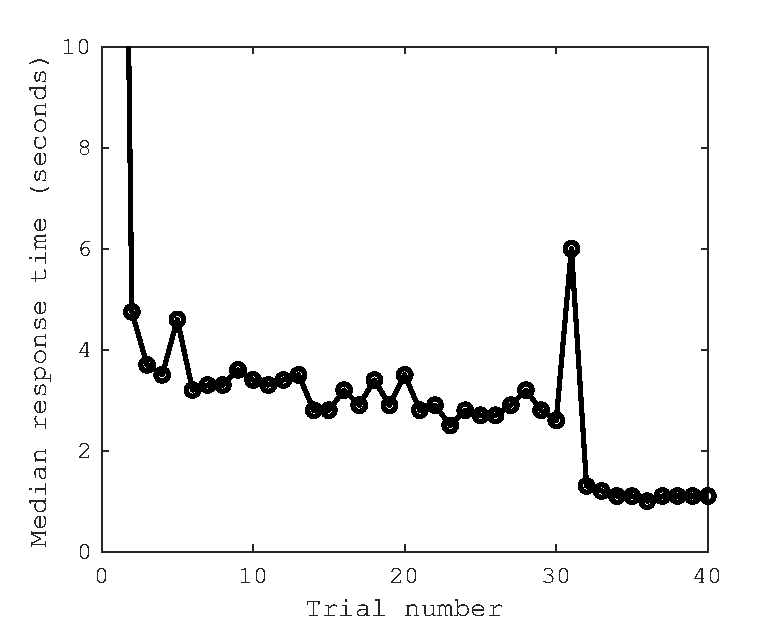
\includegraphics[max width=\textwidth]{figs/tablet/mediantime.pdf} 
\caption{Median time taken per stimulus across stimuli. Data is for all observers from Experiment 2. The point for stimulus 1 is not shown since this datapoint does not truly represent the amount of time taken by an observer. This is due to the fact that I often started the script running before approaching a participant, in order that I could start the observations without an observer seeing a white code screen on the tablet, and so in the case that the first potential participant I approached declined, this time could run into several minutes before a participant was even holding the device.}
\label{fig:mediantime}
\end{figure}

\begin{figure}[hbtp]
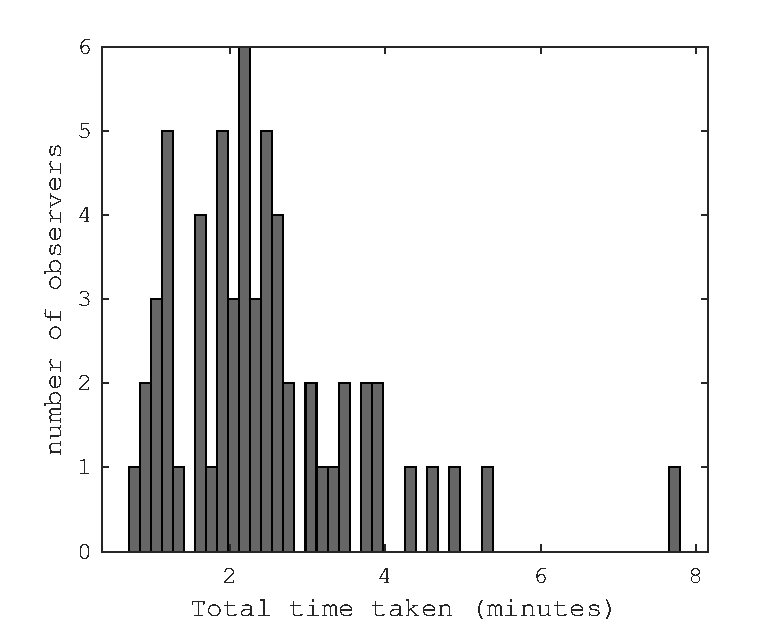
\includegraphics[max width=\textwidth]{figs/tablet/timeHistogram.pdf} 
\caption{Total time taken by observers. Data is for all observers from Experiment 2. }
\label{fig:timeHistogram}
\end{figure}

From a plot of standard deviations (Figure \ref{fig:naive}), it can be seen that whilst the participants with a large amount of experience performed well, a small number of naive participants actually performed better (assuming that SD is a valid measure of performance), whilst the remainder of participants performed almost as well with limited but notable exceptions. It is worth noting that whilst I have chosen this environment to examine (`Gallery 25: Africa Gallery') since it has the highest cross-over of individuals who can be classed as `experienced', this choice might not be ideal since the Africa Gallery represents a situation where a large amount of `smearing' may occur, since the chromaticity of the light source is far outside that selectable from the practical gamut (Figure \ref{fig:exp2}). 

\begin{figure}[hbtp]
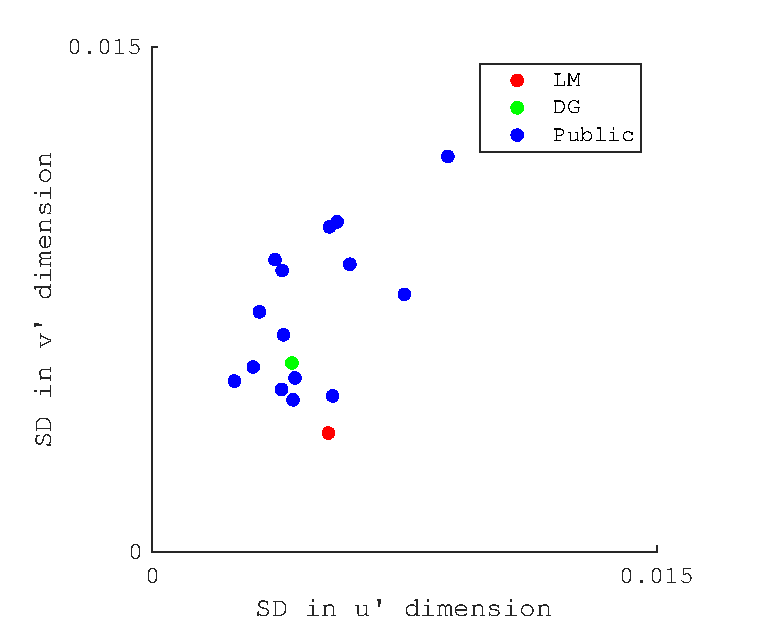
\includegraphics[max width=\textwidth]{figs/tablet/naive.pdf} 
\caption{Standard deviation in chromaticity for a subset of observers from Experiment 2 (Those from Gallery 25), highlighting data from the author and one academic supervisor (LM).}
\label{fig:naive}
\end{figure}

\subsection{Interacting with a large visual angle}

At the start of this chapter I noted the undesirable potential for the experiment to intrude upon the observer's visual world. When performing this experiment, the tablet occupies a large portion of an observer's central field of view. It should therefore be assumed that any low-level short term visual adaptation will incorporate an element of adaptation to the stimuli rather than being a pure measure of an observer's adaptational state in a particular environment. 

Regarding high level estimates of the white point, observers are aware that they are looking at a screen which they implicitly know to be an emissive device, with a white point not primarily determined by the ambient illumination. The ambiguity of the colour of the stimuli goes some way to masking the white point of the screen. If there was a clear white reference displayed on the screen I doubt we would see any distinction between environments. This is why the spatial calibration routine is run after the main trial and not before. It is possible however, that over multiple presentations of the stimuli an observer may begin to build up a representation of white which is based upon the white point of the screen. This seems particularly likely to occur when the illuminant chromaticity is far outside the practical gamut, as in Experiment 2 under the either of the strongly yellow illuminants. Under such a condition, an observer may be more likely to interpret the investigator's question as `touch the grey-est, or least colourful, point on the screen \emph{within the context of what appears on the screen over time}' rather than relating to the screen in the context of the surrounding environment.

It is possible that this effect is visible in some of our data. Looking at the results from Experiment 2 in Figure \ref{fig:exp2} it seems as though the data for 77/78 and 25 may be split into two groups (a lower and a higher group). Looking at where these fall with respect to the practical gamut, with the lower one falling centrally and the upper one falling on the slope of the practical gamut, it is possible that this distinction represents two distinct observer approaches, with the lower group tracking the white point of the screen and the upper group attempting to select the white point of the illuminant.

To mitigate this issue, some potential solutions present themselves, though most introduce new problems or exacerbate existing issues. 

The first suggestion: reduce the luminance of the display, thus directly reducing the amount of light added to the scene by the stimulus. The unwanted effect of this would be to make the stimulus more susceptible to colorimetric shift introduced by reflection of the ambient light, since this is dependent on the relative luminances of the surround and the display. Other experimenters, for example recent work reported from Anya Hurlbert's lab (VSS 2019, ICVS 2019) used a small screen device which was physically masked from the effect of the ambient illumination. Physical masking might be difficult in a situation where touch responses are desired.

The second potential solution suggested is to reduce the size of the stimulus, either by reducing the area of the screen used, or by using a physically smaller display device. The unwanted effect of this, if done crudely, would be to reduce the area of colour-space from which observers could make selections, exacerbating the `smearing' issue previously discussed. If the stimulus was redefined to consider this, such that a larger area of colour-space was presented to observers (in a smaller physical space), this would reduce the precision of the data collection, since one source of imprecision (touch input) is presumed to be relatively invariant with the size of the stimulus (thus a smaller screen would make it more of a problem.

An alternative approach might be to modify the task in some way such that the observer answered as if the tablet was a reflective device. This might be achieved by physical modifications, such that the tablet-ness of the device was obscured, or possibly through a careful modification of the question posed to the observer, à la \citet{arend_simultaneous_1986}, such that the participant was explicitly asked to pretend that they were viewing a reflective surface.

\subsection{Limitations of screen based experiments} \label{sec:bounding}

Trichromatic display devices are unable to reproduce the entire gamut of visible colour. In the case of the specific display device used here, the gamut of producible chromaticities is visually described in Figure \ref{fig:gamut}. The gamut of chromaticities actually displayed to observers, under this version of this method, is shown in Figure \ref{fig:practical}, and has been referred to using the term `practical gamut'.

As discussed in \ref{sec:limitations}, chromaticities that lie outside this gamut are consequently not available as options for a participant to select, and in the current set-up which employs random rotation and offset, the colours towards the edge of the practical gamut are displayed less frequently than those at the centre of the practical gamut, which has the practical consequence that where observers may prefer to make an achromatic selection outside this gamut, or close to the edge of it, data may exhibit `smearing'. It would be possible to see, from the analysis of data, whether an observer was constantly selecting a chromaticity on the physical edge of the display, which might be a marker of such activity. This analysis has not been completed at this time.

It is therefore not entirely correct to say that an observer's selected chromaticities will dutifully represent the observer's achromatic point. Rather, it can be said that their achromatic point is likely to fall in the direction of the vector between some objective neutral and the observed mean. There are several issues which result from this methodological limitation.

Firstly, the definition of an objective neutral point, from which such a vector could be anchored, is not a simple task. The most sensible option might be the chromaticity of the geometric centre of the stimulus (which I have referred to previously as `objective white'), which on average will be presented in the centre of the screen and most frequently. This choice is particularly tempting since this chromaticity, following our definition of the stimulus, is also the native white point of the display. However, as neat this may sound, this decision is still arbitrary to an extent however, as no true objective white point can reasonably be posited, and the white point of the display in this case bears no relation to anything other than a manufacturer decision. 

Secondly, this issue makes the results, and therefore the method, difficult to compare to previous methods. Previous comparisons between different experiments and experimental methods in this area have been achieved through comparison of `constancy indices' which describe in some way the geometrical relationship between an initial achromatic point, an adapting stimulus, and the posterior achromatic point\footnote{See \citet{foster_color_2011} for both a description of the various constancy indices in use, and a comparison across a number of studies of recorded values of constancy index.}. 

One modification to the methodology which may improve the situation, would be to render the stimuli on-the-fly (rather than calling the same stimuli for each presentation) with the observer's previous selection having some influence on the new stimulus. A simple implementation of this would be to generate stimuli following the rule that the white point of the stimuli was defined by the achromatic point of the participant's previous achromatic selection. In this way, the white point of each stimulus would, over trials, move closer to the participant's true preferred achromatic point, even if it had not been present in the initial stimuli. This would, of course, only be successful if the participant's preferred achromatic point was within the hardware gamut. 

Such schemes have been used previously, and they have been referred to as operating with an `adaptive starting rule'. \citet{delahunt_evaluation_2001} describes the process:

\begin{quote}
``\dots I used what Brainard refers to as the \emph{`adaptive starting rule'}. The a* and b* initial settings were randomized within the coordinate rectangle [-25,25] x [-25,25] centered on a reference chromaticity which was calculated as follows. For the first setting, the reference chromaticity was the white point defined by a reference illuminant. [\dots] For each subsequent setting, the reference chromaticity was the achromatic setting made in the previous setting.''
\end{quote}

Had this method been known of at the beginning of the project, it would have been implemented. I would recommend that if this method were developed further, integration of an adaptive starting rule should be considered.

Also of note is the methodology developed by \citet{smithson_colour_2004}, whereby colour boundaries are determined from categorical judgements. This type of method may be beneficial in detecting a change in chromatic adaptation even when the neutral point is out of gamut. It may also help to address the noisy nature of data collected through achromatic setting methods.

One further point of consideration which falls to be discussed within this section; the attentive reader may have noticed in some figures (e.g. Figure \ref{fig:basement_rgby_test}) that the selected achromatic points fall outside of the practical gamut. This of course represents a paradox, as participants should not have been able to select points outside of the practical gamut. The reason that this appears to occur is disappointingly mundane; whereas the practical gamut is calculated from screenshots of a set of real stimuli, and thus reports on what is actually delivered to the screen, the participant data is converted from spatial data to chromaticity data with no accounting for this, simply using the definition of the ideal stimulus prescribed at the very first stage of stimulus generation (before the practicalities of colour-space gamut restriction have had any effect).

\subsection{Impact of ipRGCs on chromatic adaptation}

Considering the lack of discernibility between data collected under the two conditions, I conclude here that we are unable to reject the null hypothesis. There are multiple reasons worthy of consideration which could make the above finding a Type II error (false negative): 

Our experimental power may be too low; considering that we have no estimate for effect size, experimental power is undetermined. However, if melanopic flux was a considerable contributor to the process of chromatic adaptation, even if I hadn't seen a distinction in the group data I may have expected to see a distinction in the individual observer data (Figures \ref{fig:PAMELA_20180205_Individual} and \ref{fig:PAMELA_20180205_Individual2}).

It is possible, considering we only ran this experiment at our chosen levels of photopic and melanopic luminances, that melanopsin may only play an active role at other luminances. If further experiments of this type were undertaken, it would be wise to match for cone catches instead of relying on chromaticity as a proxy. This would also ensure matching for luminance. Considering current knowledge regarding chromatic adaptation differing lux levels shouldn't be a concern, however it would be normal experimental procedure to equate luminance across conditions.

It is also possible that our melanopic contrast was too low - it is not an ideal comparison, but \citet{spitschan_human_2017-1} found that melanopic weber contrast above 100\% was needed to elicit a response (ours was 74\%). Equally, it is possible that both sources contained a suprathreshold level of melanopic activation, and were equally saturating the any melanopic input to colour appearance. Before further studies of this type are performed, a clear framework for the involvement of melanopsin in colour constancy is required.

Future experimenters should also consider the introduction of a third condition which was colorimetrically different, but matched for melanopic flux, in order to improve the ability to predict expected effect size. One method to decide the amount of colorimetric difference, might be to follow the `splatter' logic of \citet{spitschan_human_2016}, whereby the chromatic difference is calculated to correspond with the maximum chromatic difference resultant between two nominally metameric conditions introduced by differences between a real observer and a standard observer.

Other potential improvements to the above experimental methodology include:

\begin{enumerate}
    \item Repeating all conditions, as opposed to only one. This would improve an experimenter's ability to assess repeatability.
    \item Randomising the initial order of participants. Also, the question of whether to keep order (and thus adaptation time) the same for repeated trials is worthy of further consideration. Careful planning could allow for the parallel investigation of the effect of adaptation time.
    \item Testing for colour-anomalous vision. On balance, for clarity, it would probably be prudent for future investigators to implement an additional colour-anomalous vision test as a pre-screening, rather than relying on this experimental method as an implicit colour-vision test.
\end{enumerate}

\subsection{Coding language}

One further recommendation, for a future investigator wishing to build upon this method, or for myself should I return to it, would be to address the current situation of a split across \gls{MATLAB} and Python. The current situation arose because, having started building the software in Python (specifically PsychoPy), due to the open-source nature of that project (and the implication that those outside of academia could more easily adopt and adapt the method, as well as the fact that this program would have to run on a small tablet, which I was unsure would run \gls{MATLAB}) I found that my skills within Python were critically lacking when it came to generating colorimetrically defined imagery, and that my skills and the skills of those around me were much further advanced in \gls{MATLAB}. I mention this primarily so that any future user might not attach any false significance to the split across languages.

\section{Conclusions}

Here I have presented a development upon the established method of achromatic point setting, which would allow colour constancy experiments to be performed in real and/or complex environments. This would allow more complex questions to be asked, such as what cues observers use when there are conflicting cues, or cues that vary over space and time.

The method also has the advantage that it is quick and easy to explain to naive observers, meaning that a greater number, and broader demographic, of participants can be used compared to a traditional study. Naive observers do not seem to perform significantly worse than trained/colour-scientist observers.

The key tests for this methodology were that it presented a stable stimulus which was relatively unaffected by the ambient environment, and that it was able to record differences between an observer's achromatic settings in situations where we would expect to see differences. Having explored both of these tests I conclude that this methodology broadly satisfies both (with some caveats); the colorimetry of the display was not affected in a way that would corrupt the stimuli under the conditions considered, and under conditions where we would have expected to see a distinction in response we have indeed seen one (and vice versa).

An experiment, considering whether melanopsin activation has an influence upon white point selections, found no evidence for such. Consideration was given to the factors that could have led to a type II error in this case.

The general limitations and recommendations for further development of the method were discussed, with a particular focus on the limitations due to the static stimulus and the bounding issues that this created.

%LM: effect of handedness? Gender?


